%%%%%%%%%%%%%%%%%%%%%%%%%%%%%%%%%%%%%%%%%
% Masters/Doctoral Thesis 
% LaTeX Template
% Version 2.5 (27/8/17)
%
% This template was downloaded from:
% http://www.LaTeXTemplates.com
%
% Version 2.x major modifications by:
% Vel (vel@latextemplates.com)
%
% This template is based on a template by:
% Steve Gunn (http://users.ecs.soton.ac.uk/srg/softwaretools/document/templates/)
% Sunil Patel (http://www.sunilpatel.co.uk/thesis-template/)
%
% Template license:
% CC BY-NC-SA 3.0 (http://creativecommons.org/licenses/by-nc-sa/3.0/)
%
%%%%%%%%%%%%%%%%%%%%%%%%%%%%%%%%%%%%%%%%%

%----------------------------------------------------------------------------------------
%	PACKAGES AND OTHER DOCUMENT CONFIGURATIONS
%----------------------------------------------------------------------------------------

\documentclass[
12pt, % The default document font size, options: 10pt, 11pt, 12pt
%oneside, % Two side (alternating margins) for binding by default, uncomment to switch to one side
english, % ngerman for German
doublespacing, % Single line spacing, alternatives: onehalfspacing or doublespacing
%draft, % Uncomment to enable draft mode (no pictures, no links, overfull hboxes indicated)
%nolistspacing, % If the document is onehalfspacing or doublespacing, uncomment this to set spacing in lists to single
%liststotoc, % Uncomment to add the list of figures/tables/etc to the table of contents
%toctotoc, % Uncomment to add the main table of contents to the table of contents
%parskip, % Uncomment to add space between paragraphs
%nohyperref, % Uncomment to not load the hyperref package
headsepline, % Uncomment to get a line under the header
%chapterinoneline, % Uncomment to place the chapter title next to the number on one line
%consistentlayout, % Uncomment to change the layout of the declaration, abstract and acknowledgements pages to match the default layout
]{MastersDoctoralThesis} % The class file specifying the document structure

\usepackage[utf8]{inputenc} % Required for inputting international characters
\usepackage[T1]{fontenc} % Output font encoding for international characters
\usepackage{mathpazo} % Use the Palatino font by default
\usepackage{textcomp}
\usepackage{mathtools}
\usepackage{algorithm2e, setspace}
%\usepackage[backend=bibtex,style=authoryear,natbib=true]{biblatex} % Use the bibtex backend with the authoryear citation style (which resembles APA)

\usepackage[backend=bibtex,natbib=true]{biblatex} % Use the bibtex backend with the authoryear citation style (which resembles APA)

\addbibresource{src/references.bib} % The filename of the bibliography

\usepackage[autostyle=true]{csquotes} % Required to generate language-dependent quotes in the bibliography

%----------------------------------------------------------------------------------------
%	MARGIN SETTINGS
%----------------------------------------------------------------------------------------

\geometry{
	%paper=a4paper, % Change to letterpaper for US letter
	paper=letterpaper, % Change to letterpaper for US letter
	inner=2.5cm, % Inner margin
	outer=3.8cm, % Outer margin
	bindingoffset=.5cm, % Binding offset
	top=1.5cm, % Top margin
	bottom=1.5cm, % Bottom margin
	%showframe, % Uncomment to show how the type block is set on the page
}

%----------------------------------------------------------------------------------------
%	THESIS INFORMATION
%----------------------------------------------------------------------------------------

\thesistitle{Towards  Trusted Relational Temporal Database Using Blockchain} % Your thesis title, this is used in the title and abstract, print it elsewhere with \ttitle

\supervisor{Dr. Ken \textsc{Pu} \\ Dr. Ying \textsc{Zhu}} % Your supervisor's name, this is used in the title page, print it elsewhere with \supname
\examiner{} % Your examiner's name, this is not currently used anywhere in the template, print it elsewhere with \examname
\degree{Master of Science in Computer Science} % Your degree name, this is used in the title page and abstract, print it elsewhere with \degreename
\author{Mohammadamin \textsc{Beirami}} % Your name, this is used in the title page and abstract, print it elsewhere with \authorname
\addresses{} % Your address, this is not currently used anywhere in the template, print it elsewhere with \addressname

\subject{Computer Science} % Your subject area, this is not currently used anywhere in the template, print it elsewhere with \subjectname
\keywords{} % Keywords for your thesis, this is not currently used anywhere in the template, print it elsewhere with \keywordnames
\university{{University of Ontario Institute of Technology}} % Your university's name and URL, this is used in the title page and abstract, print it elsewhere with \univname
\department{{Faculty of Science}} % Your department's name and URL, this is used in the title page and abstract, print it elsewhere with \deptname
\group{} % Your research group's name and URL, this is used in the title page, print it elsewhere with \groupname
\faculty{} % Your faculty's name and URL, this is used in the title page and abstract, print it elsewhere with \facname

\AtBeginDocument{
\hypersetup{pdftitle=\ttitle} % Set the PDF's title to your title
\hypersetup{pdfauthor=\authorname} % Set the PDF's author to your name
\hypersetup{pdfkeywords=\keywordnames} % Set the PDF's keywords to your keywords
}

\begin{document}

\frontmatter % Use roman page numbering style (i, ii, iii, iv...) for the pre-content pages

\pagestyle{plain} % Default to the plain heading style until the thesis style is called for the body content

%----------------------------------------------------------------------------------------
%	TITLE PAGE
%----------------------------------------------------------------------------------------

\begin{titlepage}
\begin{center}

\vspace*{.06\textheight}
{\scshape\large \univname\par}\vspace{0.5cm} % University name
\textsc{\Large Master Thesis}\\[0.5cm] % Thesis type

\HRule \\[0.4cm] % Horizontal line
{\large \bfseries \ttitle\par}\vspace{0.4cm} % Thesis title
\HRule \\[1.0cm] % Horizontal line
 
\begin{minipage}[t]{0.4\textwidth}
\begin{flushleft} \large
\emph{Author:}\\
{\authorname} % Author name - remove the \href bracket to remove the link
\end{flushleft}
\end{minipage}
\begin{minipage}[t]{0.4\textwidth}
\begin{flushright} \large
\emph{Supervisors:} \\
{\supname} % Supervisor name - remove the \href bracket to remove the link  
\end{flushright}
\end{minipage}\\[2cm]
 
\vfill

\large \textit{A thesis submitted in fulfillment of the requirements\\ for the degree of \degreename}\\[0.3cm] % University requirement text
%% \groupname\\\deptname\\[2cm] % Research group name and department name
 
\vfill

{\large August, 2018}\\ % Date

    {\large Copyright \textcopyright \hspace{0.3cm} Mohammadamin Beirami, 2018}
%\includegraphics{Logo} % University/department logo - uncomment to place it
 
\end{center}
\end{titlepage}

%----------------------------------------------------------------------------------------
%	DECLARATION PAGE
%----------------------------------------------------------------------------------------

\begin{declaration}
\addchaptertocentry{\authorshipname} % Add the declaration to the table of contents
\noindent I, \authorname, declare that this thesis titled, \enquote{\ttitle} and the work presented in it are my own. I confirm that:

\begin{itemize} 
\item This work was done wholly or mainly while in candidature for a research degree at this University.
\item Where any part of this thesis has previously been submitted for a degree or any other qualification at this University or any other institution, this has been clearly stated.
\item Where I have consulted the published work of others, this is always clearly attributed.
\item Where I have quoted from the work of others, the source is always given. With the exception of such quotations, this thesis is entirely my own work.
\item I have acknowledged all main sources of help.
\item Where the thesis is based on work done by myself jointly with others, I have made clear exactly what was done by others and what I have contributed myself.\\
\end{itemize}
 
\noindent Signed:\\
\rule[0.5em]{25em}{0.5pt} % This prints a line for the signature
 
\noindent Date:\\
\rule[0.5em]{25em}{0.5pt} % This prints a line to write the date
\end{declaration}

\cleardoublepage

%----------------------------------------------------------------------------------------
%	ABSTRACT PAGE
%----------------------------------------------------------------------------------------

\begin{abstract}
\addchaptertocentry{\abstractname} % Add the abstract to the table of contents
This thesis deals with the development of a Blockchain-based framework which is built on top of a Relational Database Management System (RDBMS) to investigate the authenticity of the stored records using immutable and verifiable evidences. To do this, we proposed a mechanism to document proof of work for executive transactions on the database system in an append-only temporal log table. The temporal log tables utilize Blockchain technology for two purposes: first, to grant immutability for the stored records and second, to enable trustworthiness verifiability for the records. The objective that this dissertation is trying to achieve is to design a database system that is as open and as scalable as possible and yet non of the users of the system, regardless of their level of access to the database could conceal their activities on a database. 
Although logging the transactions along with their proof of work is very useful because it creates a source of data provenance for the database system, but the fact that they require linear time to query the historical data of records, is seen as a challenging problem. To address this issue, optimally creation of multiple snapshots for the materialization is suggested to lower the time complexity of querying for the historical records on the log tables. The proposed system supports all RDBMS systems and to achieve its objectives, the system solely rely on verifiable evidences and not on putting trust on the users of the system.

\end{abstract}

%----------------------------------------------------------------------------------------
%	ACKNOWLEDGEMENTS
%----------------------------------------------------------------------------------------

\begin{acknowledgements}
\addchaptertocentry{\acknowledgementname} % Add the acknowledgements to the table of contents
This thesis owes its existence to the help, support and inspiration of several people. Firstly, I would like to express my sincere gratitude to professor Ken Pu and professor Ying Zhu my advisors, for their supports, understanding, patience, enthusiasm and encouragement and for pushing me further than I thought I could go. I would also like to thank professor Jaroslaw Szlichta and professor Ming Dong for their assistance and suggestions to write this thesis.
I wish to take this opportunity to express my sincere and particular appreciation to my family for their unflagging love, tremendous support and unconditional encouragement throughout my life and my studies. 
\end{acknowledgements}

%----------------------------------------------------------------------------------------
%	LIST OF CONTENTS/FIGURES/TABLES PAGES
%----------------------------------------------------------------------------------------

\tableofcontents % Prints the main table of contents

\listoffigures % Prints the list of figures

\listoftables % Prints the list of tables

%----------------------------------------------------------------------------------------
%	ABBREVIATIONS
%----------------------------------------------------------------------------------------

%\begin{abbreviations}{ll} % Include a list of abbreviations (a table of two columns)
%
%\textbf{LAH} & \textbf{L}ist \textbf{A}bbreviations \textbf{H}ere\\
%\textbf{WSF} & \textbf{W}hat (it) \textbf{S}tands \textbf{F}or\\
%
%\end{abbreviations}

%----------------------------------------------------------------------------------------
%	PHYSICAL CONSTANTS/OTHER DEFINITIONS
%----------------------------------------------------------------------------------------

%\begin{constants}{lr@{${}={}$}l} % The list of physical constants is a three column table
%
%% The \SI{}{} command is provided by the siunitx package, see its documentation for instructions on how to use it
%
%Speed of Light & $c_{0}$ & \SI{2.99792458e8}{\meter\per\second} (exact)\\
%%Constant Name & $Symbol$ & $Constant Value$ with units\\
%
%\end{constants}

%----------------------------------------------------------------------------------------
%	SYMBOLS
%----------------------------------------------------------------------------------------

%\begin{symbols}{lll} % Include a list of Symbols (a three column table)
%
%$a$ & distance & \si{\meter} \\
%$P$ & power & \si{\watt} (\si{\joule\per\second}) \\
%%Symbol & Name & Unit \\
%
%\addlinespace % Gap to separate the Roman symbols from the Greek
%
%$\omega$ & angular frequency & \si{\radian} \\
%
%\end{symbols}

%----------------------------------------------------------------------------------------
%	DEDICATION
%----------------------------------------------------------------------------------------

%\dedicatory{For/Dedicated to/To my\ldots} 

%----------------------------------------------------------------------------------------
%	THESIS CONTENT - CHAPTERS
%----------------------------------------------------------------------------------------

\mainmatter % Begin numeric (1,2,3...) page numbering

\pagestyle{thesis} % Return the page headers back to the "thesis" style

% Include the chapters of the thesis as separate files from the Chapters folder
% Uncomment the lines as you write the chapters

\newtheorem{prop}{Proposition}
\newtheorem{defn}{Definition}
\newtheorem{remark}{Remark}
\newtheorem{note}{Note}
\newtheorem{theorem}{Theorem}

\chapter{Motivation and Problem Definition} \label{ch:motivation}

	\section{Motivation} \label{sec:motivation}
		Historical data is widely analysed for a lot of purposes such as making data-driven decisions \cite{rose2016datascience}. Historical data could be financial reports, project data, emails, audit logs or any similar documents which contain past occurrences in an organization.

		Historical data of a database provides data provenance which makes it possible to investigate the origin, the cause and the time of the processes that made changes to the tables and records ever exsisted in a database \cite{cheney2009provenance}. This data could be collected by auditing all the transactions that occur on a database system and store them in a logfile \cite{ghoshal2013provenance}. Although in large database systems, storing these historical data could seem burdensome and impractical due to the size they may get into \cite{crosby2009tamper-evident}, but current big data technologies such as cloud storages has made it possible to store these information in an easier and more affordable way than before \cite{talia2015dataanalysis}. In practice, not only these logfiles are useful assets that could be analyzed to detect maliciously manipulated data by outsider adversaries, but they can also give a valuable insight into the activities of the privileged users on a database system \cite{sinha2014continuous}.

		Utilizing logfiles as the source of data provenance gives us a useful tool to establish a trustworthy database environment \cite{viglas2013DataProvenance}, however this requires to make sure that the records in the logfile are trusted themselves \cite{Dai2008anapproach}.The challenge is that these files are not immune from being compromised \cite{wagner2018detect}\cite{lin2015secure}. In fact, not only the inherent security tools of most of the database management systems including the relational database management system (RDBMS) has proven to be vulnearable to complex cyber-security attacks \cite{wanger2017carving}, but also the malicious activities of the insiders who can bypass all the security requirements can add up to the complexity of the problem \cite{wagner2018detect}.

		For a better understanding of the complexity of malicious attacks on the log files, consider a scenario in which a database super-user who acts as root can perform a lot of administrative tasks on a relational database. Since the super-user can bypass all the security requirements, they can remove the trace of their malicious activities from the log file. Such attempts results in the maliciously altered data in the database that are hard to identify because there are no evidences to contradict their legitimacy.
		
		The afformentioned example clearly proves that restricting the activities of the users or utilizing preventive security tools for the database system cannot guarantee that the records will always remain trustworthy. Therefore, there is a need of a mechanism that makes the complexity of creating undetectable forgeries on the data provenance sources extremely expensive and unimaginable for all the users regardless of their level of accessibility to the system. The system should also be able to detect any malicious or accidental data manipulation on the database solely by relying on the verifiable evidences.

		Our objective is to design a mechanism based on relational database management system that provides trustworthy logfiles that are used as the source of data provenance of the database system. To achieve the objective of both providing trusted data and a functional system, we argue that the following requirements need to be addressed.

		\begin{itemize}
			  \item \textbf{\textit{Immutability of the records:}} To make sure that the a record in a relational database is trustworthy, performing undetectable malicious modification on that record should be extremely expensive. That is, any malicious or accidental attempts to modify the records stored in a database should result in an evident inconsistency in the data stored.

			  \item \textbf{\textit{Verifiability of trustworthiness:}} For all the records that are submitted in a database system, the origin of that transaction as well as the ligitimacy of the origin should be investigatbale using the verifiable evidences .

			  \item \textbf{\textit{Fast querying:}} The tables that contain historical records can become extremely large, and as a result, querying on these tables and verifying the trustworthiness of the result of queries can become inefficient \cite{crosby2009tamper-evident}\cite{beirami2018snapshot}. For the system to be functional, a mechanism should be implemented in order to reduce the cost of both answeing to the queries and verifying the trustworthiness of the query results.

			  \item \textbf{\textit{Fast appending:}} The system needs to collect all the security information of the transactions and append them to the logfile in an immutable way. In order to create a functional system, this process should be done as cheap as possible.
	\end{itemize}
		In this thesis, our research is focused on the relational databases that are as open and as scalable as possible. We assume that the adversaries are present and do malicious activities on the network, however our goal is to make their attempt to forge the records extremely expensive and evident. We believe that our proposed system is powerful in the sense that it removes the user-based trust and testifies the credibility or invalidity of the records by analyzing verifiable evidences. The system is able to detect privileged database misuses such as altering the auditing mechanism or manipulating the historical data. Our system utilizes many native to RDBMS tools such as relational temporal tables to store the historical data and cryptographic techniques to make transactions immutable and verifiable, therefore it could be supported by all RDBMSes available today with least additional requirements.


\chapter{Background and Related Work}


\begin{itemize}
    \item General purpose description of temporal databases and its usage
    \item Blockchain
\end{itemize}

Related work

\begin{itemize}
    \item citations
    \item description of what has been done.
\end{itemize}

\chapter{Problem Definition and Algorithms}

In this chapter, we fomally define the problem of large query workload inefficiency in the context of temporal relational databases and then we propose a solution to lower the cost of such queries. In the next stage, we offer a practical procedure to implement the Blockchain methodology as well as the principles to add and verify trustworthiness of the records using Blockchain in a temporal relational database.

\section{Problem definition}
Keeping the historical records of transactions on a database system is useful because it stores the entire updates of a database. In our proposed system these historical records could be used to regenerate the form of a table (snapshot) or a record in a specific timestamp. Also, cryptographic techniques could be used to create a cryptographic chain in order to secure these records from tampering, therefore by investigating the authenticity of all transactions applied to an specific record throughout its lifecycle, the trustworthiness of that record could be ensured. Append-only temporal relational tables, if chosen for keeping the historical records, are beneficial because not only they are simple to implement, but also there is the luxary of having RDBMS to manage and perform queries on such tables.

\begin{example}
	Definition of a timeline was introduced in Definition \ref{dfn:timeline}. The historical records obtained from auditing the database transaction could be seen as a timeline. A request to regenerate the form of a table (snapshot) or a record can be depicted in \ref{fig:snapshot_notion}
\label{example:timeline}
\end{example}

\begin{figure}
	\centering
	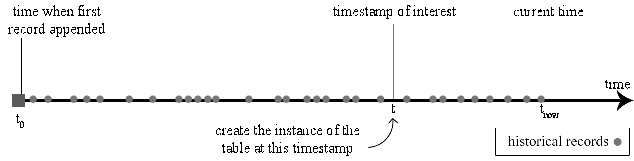
\includegraphics[width=\textwidth]{figs/snapshot_notion.pdf}
	\caption{The notion of creating snapshot on the timeline.}
	\label{fig:snapshot_notion}
\end{figure}


\begin{prop}[Linear time in creating snapshots]
	The notion of creating a snapshot that shows the instance of the table $r$ in a certain timestamp $t$, using historical records stored in an append-only temporal relational table $r^T$ defined in \textbf{Definition 5}. Assume that the tables were updated at a constant rate over time, then the complexity of $\mathrm{snapshot}(r, t)$ is $$\mathcal{O}(|\{x: x\in r^T\mathrm{\ and\ } x.\mathrm{updates} \leq t\}|)\simeq \mathcal{O}(t)$$ 
	Since $r^T$ could be seen as a timeline, the records which need to be checked can be depicted in \ref{fig:checked_records}. This clearly indicates that a linear time is required to compute a snapshot at a timestamp of interest and as the size of $r^T$ grows in size, creating snapshot become computationally more expensive.
\label{prop:linear_time}
\end{prop}

\begin{figure}[b]
	\centering
	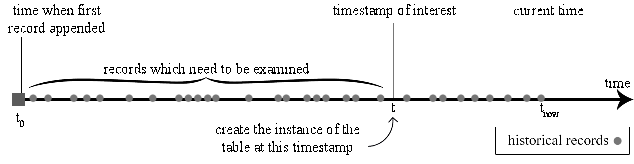
\includegraphics[width=\textwidth]{figs/tobechecked_records.pdf}
	\caption{The records which needs to be checked when creating a snapshot.}
	\label{fig:checked_records}
\end{figure}

\begin{example}
	Given a normal relational table $r_1$ (Table \ref{table:normal_table_2}) and a temporal relational table $r_1^T$ (Table \ref{table:temporal_table_2}) which contains the historical data of $r_1$, the $r_1$ at $t=2018-04-01$ looked like Table $\ref{table:normal_table_2_t}$
\label{example:snapshot_table}
\end{example}

\begin{center}
\begin{table}[t]
	\centering
	\caption{Normal Relational Table $r_1$}
	\label{table:normal_table_2}
	\begin{tabular}{p{4cm}p{4cm}p{4cm}}
		\hline
		id & item      & value  \\ \hline
		22 & Pencil    & 7.50 \\
		23 & Notebook & 12.0   \\ 
		24 & Console & 230.0 \\ \hline
	\end{tabular}
\end{table}

\begin{table}[t]
	\centering
	\caption{Temporal Table $r_1^T$}
	\label {table:temporal_table_2}
	\begin{tabular}{p{1cm}p{2cm}p{3cm}p{3cm}p{2cm}}
		\hline
		id & item      & value  & updated  & deleted\\ \hline
		21 & Ruler    & 3.25  & 2018-02-10  &  - \\  
		22 & Pencil    & 8.0  & 2018-03-21  &  - \\
		22 & Pencil    & 9.0  & 2018-03-30  &  -\\
		23 & Notebook & 11.0  & 2018-04-01 & - \\
		22 & Pencil & 6.0  & 2018-04-01 & - \\
		21 & Ruler    & 3.25  & -  &  2018-04-02 \\
		23 & Notebook & 12.0  & 2018-04-02 & - \\ 
		22 & Pencil & 7.50  & 2018-04-05 & - \\ 
		24 & Console & 230.0  & 2018-04-05 & - \\ \hline
	\end{tabular}
\end{table}
\end{center}
\begin{center}
\begin{table}
	\centering
	\caption{Normal Relational Table $r_1$ at t = 2018-04-01}
	\label{table:normal_table_2_t}
	\begin{tabular}{p{4cm}p{4cm}p{4cm}}
		\hline
		id & item  & value  \\ \hline
		21 & Ruler & 3.25 \\
		22 & Pencil & 6.0   \\ 
		23 & Notebook & 11.0 \\ \hline
	\end{tabular}
\end{table}
\end{center}

\subsection{Query answering using snapshots} 
Using pre-computed materialized view has been proven to be effective in reducing the computational time of query answering \cite{sohrabi2016materialized} \cite{du2017deepsea}. Since running queries $Q(t)$ on temporal table $r^T$ to build snapshots or generate latest version of a record at a timestamp of interest requires linear time with time complexity of approximately $\mathcal{O}(t)$, consequently in the presence of multiple and concurrent queries, such transactions are computationally expensive and inefficient. We argue that, if a snapshot is computed at the timestamp $t$ and placed on the timeline, the computational time of answering to the subsequent queries on $r^T$ is reduced. The notion of having precomputed snapshots for materialization can be depicted as Figure \ref{fig:snapshot_materialization}. Note that the snapshot could exist before or after a query and in both cases, the query can use the snapshot for materialization.

\begin{figure}[t]
	\centering
	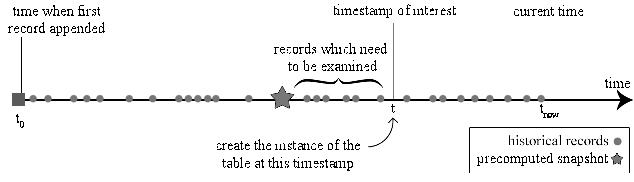
\includegraphics[width=\textwidth]{figs/snapshot_materialization.pdf}
	\caption{The records which needs to be checked when creating a snapshot with having a precomputed snapshot for materialization.}
	\label{fig:snapshot_materialization}
\end{figure}

\begin{prop}
	suppose we have a materialized snapshot $snapshot(r,s)$. Then $snapshot(r,t)$ can be computed with complexity:
	$$\mathcal{O}(|\{x: x\in r^T\mathrm{\ and\ } x.\mathrm{updates} \in [s,t]\}|) \simeq \mathcal{O}(|s-t|)$$
\label{prop:materialized_snapshot_complexity}
\end{prop}

\begin{example}
	Given a temporal relational table $r_1^T$ (Table \ref{table:temporal_table_3}) and a precomputed snapshot table $s_1$ at timestamp $t = 2018-03-11$(Table \ref{table:snapshot_s1}), we are interested to create a snapshot $s_2$ which is the instance of table $r_1$ at the timestamp of $t = 2018-03-15$. In order to compute snapshot $s_2$, Table \ref{table:transactions_nonmaterialized} shows the transactions which needs to be evaluated without using snapshot $s_1$ and Table \ref{table:transactions_nonmaterialized} is when $s_1$ is used for materialization. This example clearly shows that when creating snapshot $s_2$ (Table \ref{table:snapshot_s2}), less transactions need to be evaluated when $s_1$ is used for materialization.
\label{example:materialized_snapshot_complexity}
\end{example}

\begin{center}
\begin{table}
	\centering
	\caption{Temporal Table $r_1^T$}
	\label {table:temporal_table_3}
	\begin{tabular}{p{1cm}p{2cm}p{3cm}p{3cm}p{2cm}}
		\hline
		id & item & value  & updated  & deleted\\ \hline
		1 & Paper & 0.25  & 2018-02-10  &  - \\  
		2 & Scissors & 8.0  & 2018-02-12  &  - \\
		3 & Folder & 1.50  & 2018-02-12  &  - \\
		1 & Paper & 0.30  & 2018-02-13  &  - \\
		4 & Pencil & 3.0  & 2018-02-16  &  - \\
		3 & Folder & 1.75  & 2018-02-21  &  - \\
		5 & Batteries & 8.0  & 2018-02-23  &  - \\
		1 & Paper & 0.35  & 2018-02-25  &  - \\
		6 & Notebook & 7.0  & 2018-03-01  &  - \\
		5 & Batteries & 9.0  & 2018-03-01  &  - \\
		4 & Pencil & 3.25  & 2018-03-04  &  - \\
		1 & Paper & 0.35  &  - &  2018-03-04 \\
		7 & Ruler & 4.0  & 2018-03-06  &  - \\
		2 & Scissors & 8.50  & 2018-03-07  &  - \\
		7 & Ruler & 4.50  & 2018-03-08  &  -\\
		5 & Batteries & 11.0  & 2018-03-10 & - \\
		3 & Folder & 1.75  & - & 2018-03-11 \\
		7 & Ruler & 4.50  & -  &  2018-03-12 \\
		6 & Notebook & 7.50  & 2018-03-15 & - \\ 
		2 & Scissors & 7.50  & 2018-03-17 & - \\ \hline
	\end{tabular}
\end{table}
\begin{table}
	\centering
	\caption{Snapshot $s_1$ at $t = 2018-03-11$}
	\label{table:snapshot_s1}
	\begin{tabular}{p{4cm}p{4cm}p{4cm}}
		\hline
		id & item  & value  \\ \hline
		2 & Scissors & 8.5   \\ 
		4 & Pencil & 3.25   \\ 
		5 & Batteries & 11.0   \\ 
		6 & Notebook & 7.0 \\ 
		7 & Ruler & 4.50   \\ \hline
	\end{tabular}
\end{table}
\end{center}

\begin{center}
\begin{table}
	\centering
	\caption{the transactions to compute snapshot $s_2$ at $t = 2018-03-15$ without using snapshot $s_1$ for materialization}
	\label{table:transactions_nonmaterialized}
	\begin{tabular}{p{1cm}p{2cm}p{2cm}p{3cm}p{2cm}p{2cm}}
		\hline
		id & item & Transaction  &timestamp & value  &query on\\ \hline
		1 & Paper & cretaed & 2018-02-10 & 0.25 & $r_1^T$ \\
		  & Paper & updated & 2018-02-13 & 0.30 & $r_1^T$ \\
		  & Paper & updated & 2018-02-25 & 0.35 & $r_1^T$ \\
		  & Paper & deleted & 2018-03-04 & - & $r_1^T$ \\ \hline
		2 & Scissors & cretaed & 2018-02-12 & 8.0 & $r_1^T$ \\
		  & Scissors & updated & 2018-03-07 & 8.50 & $r_1^T$ \\ \hline
		3 & Folder & cretaed & 2018-02-12 & 1.50 & $r_1^T$ \\
		  & Folder & updated & 2018-02-21 & 1.75 & $r_1^T$ \\
		  & Folder & deleted & 2018-03-11 & - & $r_1^T$ \\ \hline
	  	4 & Pencil & cretaed & 2018-02-16 & 3.0 & $r_1^T$ \\
		  & Pencil & updated & 2018-03-04 & 3.25 & $r_1^T$ \\ \hline
  	  	5 & Batteries & cretaed & 2018-02-23 & 8.0 & $r_1^T$ \\
		  & Batteries & updated & 2018-03-01 & 9.0 & $r_1^T$ \\
		  & Batteries & updated & 2018-03-10 & 11.0 & $r_1^T$ \\ \hline
		6 & Notebook & cretaed & 2018-03-01 & 7.0 & $r_1^T$ \\ 
		  & Notebook & updated & 2018-03-15 & 7.50 & $r_1^T$ \\ \hline
		7 & Ruler & cretaed & 2018-03-06 & 4.0 & $r_1^T$ \\
		  & Ruler & updated & 2018-03-08 & 4.50 & $r_1^T$ \\
		  & Ruler & deleted & 2018-03-12 & - & $r_1^T$ \\ \hline

	\end{tabular}
\end{table}
\end{center}

\begin{center}
\begin{table}
	\centering
	\caption{the transactions to compute snapshot $s_2$ at $t = 2018-03-15$ using snapshot $s_1$ for materialization}
	\label{table:transactions_materialized}
	\begin{tabular}{p{1cm}p{2cm}p{2cm}p{3cm}p{2cm}p{2cm}}
		\hline
		id & item & Transaction  &timestamp & value  &query on\\ \hline
		2 & Scissors & - & - & 8.50 & $s_1$ \\ \hline
	  	4 & Pencil & - & - & 3.25 & $s_1$ \\ \hline
  	  	5 & Batteries & - & - & 11.0 & $s_1$ \\ \hline
		6 & Notebook & - & - & 7.0 & $s_1$ \\ 
		  & Notebook & updated & 2018-03-15 & 7.50 & $r_1^T$ \\ \hline
		7 & Ruler & - & - & 4.50 & $s_1$ \\
		  & Ruler & deleted & 2018-03-12 & - & $r_1^T$ \\ \hline
	\end{tabular}
\end{table}
\end{center}

\begin{center}
\begin{table}
	\centering
	\caption{Snapshot $s_2$ at $t = 2018-03-15$}
	\label{table:snapshot_s2}
	\begin{tabular}{p{4cm}p{4cm}p{4cm}}
		\hline
		id & item  & value  \\ \hline
		2 & Scissors & 8.50   \\ 
		4 & Pencil & 3.25   \\ 
		5 & Batteries & 11.0   \\ 
		6 & Notebook & 7.50 \\ \hline
	\end{tabular}
\end{table}
\end{center}

\subsection{Optimal materialization of snapshots}
Let $T_q = \{q_1, q_2, \dots, q_n :q_i \in \mathcal{T}\}$ be the timestamps of $n$ queries, each querying the database at $D^T(q_i)$. To save on computational cost in answering the queries on temporal database $D^T$, we propose to compute $m$ number of snapshots $snapshot_j(r,t)$ in optimal timestamps on the timeline to answer to $T_q$ at lowest possible cost. The cost function is defined as the total query answering cost given $m$ number of precomputed snapshots. Note that $m$ is defined based on available resources in the system.

\begin{defn}[Cost of Query Answering] 
	In the presence of a single materialized precomputed snapshot at timestamp $s \in \mathcal{T}$, the cost of answering the query $T_q$ is calculated as:
	$$\mathrm{cost}(T_q | s) = \sum_{q\in T_q} |q - s|$$
	Now if multiple snapshots at timestamps $S=\{s_1, s_2, \dots, s_m : s_j \in \mathcal{T}\}$ were precomputed and materialized, then 
	$$\mathrm{cost}(T_q|S) = \sum_{q\in T_q} \min\{|q-s| : s\in S\}$$
\label{defn:cost_of_query_answering}
\end{defn}

\begin{defn}[Optimal Snapshot placement]: 
    For the \emph{single snapshot placement} problem, the goal is to find the timestamp $s^*$ such that 
	$$cost(T_q|s)= Arg min(\sum_{q\in T_q}|q - s|)$$

	The \emph{$m$-snapshot placement} problem is to compute $m$ number of timestamps $S^*=\{s_1, s_2, \dots, s_m: s_j \in \mathcal{T}\}$ to place $m$ number of snapshots for materialization, such that 
	$$cost(T_q|S)= Arg min(\sum_{q\in T_q}\{|q - s|:s \in S\})$$
\label{defn:optimal_snapshot_placement}
\end{defn}

In the subsequent sections, we present the algorithms to address the problem of snapshot placement.

\section{Optimal single snapshot placement}
We begin solving the problem of snapshot placement by first finding the optimal timestamp for a single snapshot. Let $T_q^* = {q_1,q_2, \dots , q_n}$ be $n$ number of queries performed on the temporal database. $T_q^*$ gives us a valuable insight into the query patterns on the temporal database, that could be used to find optimal position of snapshots.

\begin{prop}
	Given the performed queries $T_q^*$, the optimal position for a single snapshot on the timeline for materialization is $s^*(T_q^*)=median(T_q^*)$ that can be computed in $\mathcal{O}(|T_q^*|)$. 
\label{prop:compute-median}
\end{prop}
    
Figure \ref{fig:optimal_materialization} shows the notion of placing snapshot in the median of queries for materialization.

\begin{figure}
	\centering
	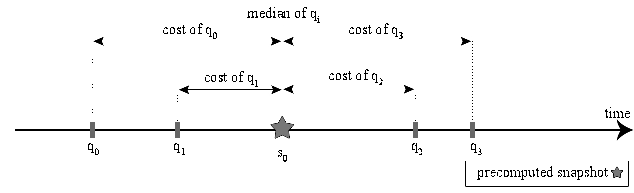
\includegraphics[width=\textwidth]{figs/optimal_materialization.pdf}
	\caption{Placing a single snapshot in the median of queries guarantees the optimal cost of query answering.}
	\label{fig:optimal_materialization}
\end{figure}

\textbf{\emph{Proof of the Proposition~\ref{prop:compute-median}}}:
	At first, we solve the problem of a single snapshot placement for two queries, and then we generalize the conclusion for multiple queries:

	Assume that there are two queries $T_q=\{q_1,q_2\ : q_i \in \mathcal{T}\}$ on the timeline, such that, $q_1<q_2$. for the placement of a single snapshot $s^* \in \mathcal{T}$ on the timeline, there are several cases which needs to be considered:

	\emph{Case 1}:
	$s^* \in [q_1,q_2]$, hence $q_1\leq s^*\leq q_2$.
	in this case, the cost is:

	$$cost(T_q|s^*)=\sum_{i=1}^2|q_i-s^*| = (s^*-q_1+q_2-s^*)=(q_2-q_1)$$

	from case 1, we can infer that the cost of running two queries $q_1$ and $q_2$ when the snapshot is placed between them, is equal to the deviation between the two queries.

	\emph{Case 2}:
	$s^* \notin [q_1,q_2]$ and $s^* < q_1 < q_2$. for this case the cost could be calculated as follows:
	$$cost_T(T_q|s^*)=\sum_{i=1}^2|q_i-s^*| = (q_1-s^*+q_2-s^*)=(q_1+q_2-2s^*) $$$$>(q_1+q_2-2q_1)=(q_2-q_1)$$

	Therefore we conclude that if the snapshot $s^*$ is placed before queries $T_q$, the cost to perform both queries is greater than when the snapshot is placed between the two queries.

	\emph{Case 3}:
	$s^* \notin [q_1,q_2]$ and $q_1 < q_2 < s^*$.
	$$cost(T_q|s^*)=\sum_{i=1}^2|q_i-s^*| = (s^*-q_1+s^*-q_2)=(2s^*-q_1-q_2) $$$$>(2q_2-q_1-q_2)=(q_2-q_1)$$

	hence, if the snapshot $s^*$ is placed after the queries $T_q$, then the cost of performing those queries are greater than when the snapshot is placed between them.

	From case1, case2 and case3, we can conclude that the optimal timestamp on the timeline that we can place the single snapshot $s^* \in \mathcal{T}$ to perform two queries $T_q = \{q_1,q_2:q_i\in \mathcal{T}\}$, where $q_1<q_2$ is when $s^* \in [q_1,q_2]$, meaning that $q_1 \leq s^* \leq q_2$, where the cost is equal to $q_2-q_1$.

	Now, we generalize our conclusion from the cases that we evaluated, for the placement of a single snapshot in the presence of $n$ number of queries on the timeline: 

	Suppose that there is a set of queries $T_q=\{q_1,q_2,...,q_n:q_i \in \mathcal{T}\}$ performed on the timeline. To evaluate the most optimal position to place the single snapshot $s^* \in \mathcal{T}$ for materialization, we breakdown the set of queries into the set of nested intervals $[q_1,q_n],[q_2,q_{n-1}],...,[q_i,q_{n+1-i}]$ where $n$ is the number of queries on timeline and $i=0,1,2,...,c$ where $c=\frac{n+1}{2}$ for odd number of queries and $c=\frac{n}{2}$ for even number of queries present on the timeline.

	Based on the conclusion that we obtained from examining case 1, case 2 and case 3 earlier, for each nested interval, the cost of queries inside them is minimized if snapshot $s^*$ is placed in a middle of the interval. Therefore if the snapshot is placed in a position which $s^*\in \{ [q_1,q_n] \wedge [q_2,q_{n-1}] \wedge ... \wedge [q_i,q_{n+1-i}] \}$ the overall cost for all queries is minimized. In other words, if the snapshot is placed in a position that is in the middle of all nested intervals, then the total sum of absolute deviation of the snapshot from all queries is minimized. The placement of snapshot $s^*$ in the median position of $T_q$ guarantees that the snapshot is placed in the middle of all nested query intervals, where the cost of queries is calculated as follows:
	$$cost(T_q|s^*)=\sum_{i=1}^n |q_i-s^*| = $$
	$$[(|q_1-s^*|+|q_n-s^*|)+(|q_2-s^*|+|q_{n-1}-s^*|)+...+|q_c-s^*|+|q_{n+1-c}-s^*|)]=$$
	$$[(s^*-q_1+q_n-s^*)+(s^*-q_2+q_{n-1}-s^*)+...+(s^*-q_c+q_{n+1-c}-s^*)]=$$
	$$[(q_n-q_1)+(q_{n-1}-q_2)+...+(q_{n+1-c}-q_c)]$$\\
	where parenthesis indicate the deviation from endpoints for one of nested intervals. In the case when there are odd number of queries performed on the timeline, the innermost interval is $[q_{\frac{n+1}{2}},q_{\frac{n+1}{2}}]$ and the position of $q_{\frac{n+1}{2}}$ is the optimal position to place snapshot $s^*$. also when there are even number of queries the innermost interval is $[q_{\frac{n}{2}},q_{\frac{n}{2}+1}]$, therefore if we choose snapshot $s^*$'s position to be at $q_{\frac{n}{2}}\leq s^*\leq q_{\frac{n}{2}+1}$,it guarantees that the snapshot exists inside each of nested intervals, and hence the sum of absolute deviation is minimized. 


\section{Optimal multiple snapshot placement}
In the presence of thousands of queries on a temporal database with millions of records, having a single snapshot reduces the cost of query answering but it is still not enough. Therefore, to reduce the overall cost of query answring, optimal timestamps should be computed on the timeline of the temporal database to place snapshots for materialization. In the following section, different approaches to compute the optimal positions on the timeline are discussed.

\begin{prop}[Segmentation of queries] 
	Given an ordered set of snapshot timestamps $S=\{s_1,s_2,...,s_m:s_i \in \mathcal{T}\}$, such that $s_i \leq s_{i+1}$, and $n$ number of queries $Q = \{q_1,q_2,...,q_n: q_i \in \mathcal{T}\}$, snapshots create $m$ number of non-overlapping segments on the queries $Q[1,i_1],Q[i_1+1,i_2],...,Q[i_{m-1},i_m]$ such that queries in the segment $Q[i_j,i_{j+1}]$ use $s_j$ to answer the queries in the optimal query answering strategy.
\label{prop:segmentation_of_queries}
\end{prop}
The notion of creating segmentations is depicted in Figure \ref{fig:segmentation}.

\begin{figure}
	\centering
	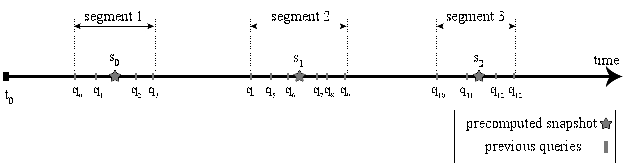
\includegraphics[width=\textwidth]{figs/segmentations.pdf}
	\caption{The notion of creating segmentations on the timeline and placing snapshot for each segmentation.}
	\label{fig:segmentation}
\end{figure}

\subsection{A recursive algorithm for optimal snapshot placements}

Let $\mathrm{opt}(Q, m)$ be the optimal $m$-snapshot placements for the query workload $Q$. Denote $Q[i,j] = \{q_i,q_{i+1},...,q_{j-1},q_j\}$.

\begin{prop}[Optimality of sub-problems]
	Let $S^* = \mathrm{opt}(Q, m)$.  Let $\mathcal{Q}$ be the partition of segments created by $S^*$.  Then, the prefix of $S^*$ is also an optimal $m-1$ snapshot placement of the prefix of $\mathcal{Q}$. Formally, $$\mathrm{prefix}(S^*) = \mathrm{opt}(\cup\mathrm{prefix}(\mathcal{Q}), m-1)$$
\label{prop:optimality_of_subproblems}
\end{prop}

\subsection{recursive approach to find optimal segmentations of the timeline}
We can formulate a recursive definition of $\mathrm{opt}(Q, m)$ using Proposition~\ref{prop:optimality_of_subproblems}. The intuition is that we try out all possible {\em last} segment of $Q$, and pick the one with the lowest cost.

The recursive definition of $\mathrm{opt}(Q, m)$ is given as:

\begin{itemize}
	\item Base case $ \mathrm{opt}(Q, 1) = \{\mathrm{median}(Q)\}$.
	\item Induction on $m$:
	$$i^* = \mathrm{argmin}\{\mathrm{cost}(\mathrm{opt}(Q[1,i], m-1)): i\in[1,
	n]\}$$
	$$
	\mathrm{opt}(Q, m) = \mathrm{opt}(Q[1, i^*]) \cup \{\mathrm{median}(Q[i^*+1, n])
	$$
\end{itemize}
The recursive formulation of $\mathrm{opt}(Q, m)$ requires $\mathcal{O}(2^{m})$.

\begin{example}
	Given the queries $Q=\{q_1=2,q_2=4,q_3=9,q_4=11,q_5=17,q_6=20\}$ (Figure \ref{fig:example_recursive_queries}) and maximum number of snapshots $m=3$, the goal is to find the most optimal segmentations using recursive algorithm to place snapshots for materialization. The steps to compute $m$ number of optimal segmentations is shown in Figure \ref{fig:example_recursive_steps}. In this example, the most optimal segmentation possible for 3 snapshots is when $segment_1 = \{q_0,q_1\}$, $segment_2 = \{q_2,q_3\}$, $segment_3= \{q_4,q_5\}$ where the total cost is 7 units. Figure \ref{fig:example_recursive_segmentation}.
\label{example:recursive_segmantation}
\end{example}

\begin{figure}[b]
	\centering
	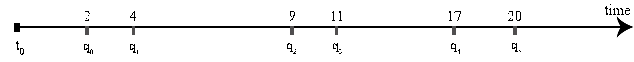
\includegraphics[width=\textwidth]{figs/example_recursive_q.pdf}
	\caption{The quer on the timeline in Example.}
	\label{fig:example_recursive_queries}
\end{figure}

\begin{figure}
	\centering
	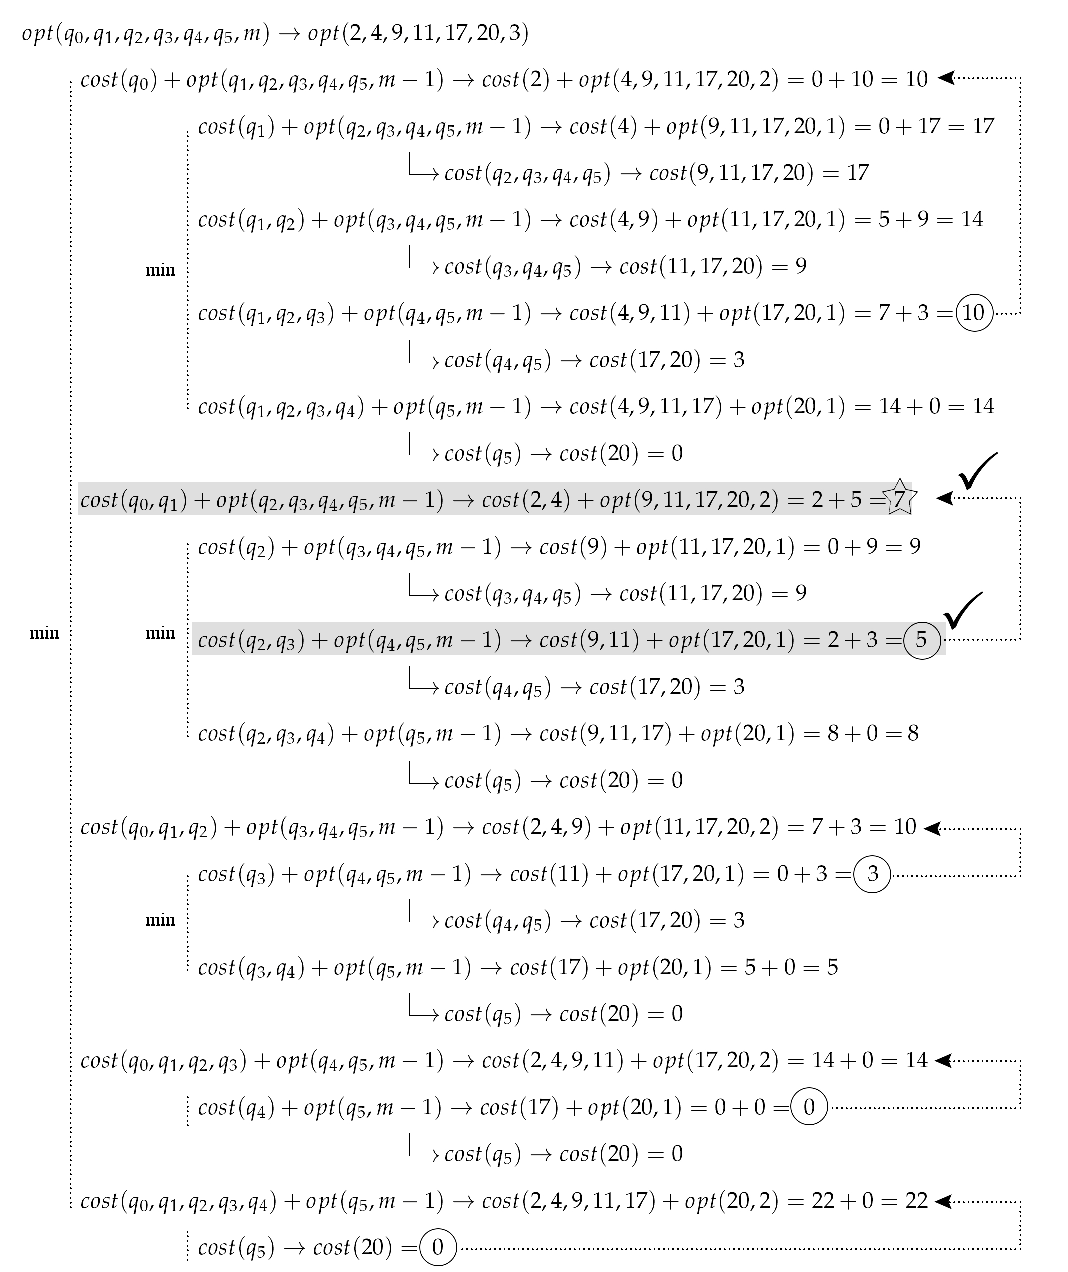
\includegraphics[width=\textwidth]{figs/recursion_example.pdf}
	\caption{Recursive approach to compute optimal segmentations for 3 snapshots.}
	\label{fig:example_recursive_steps}
\end{figure}


\begin{figure}
	\centering
	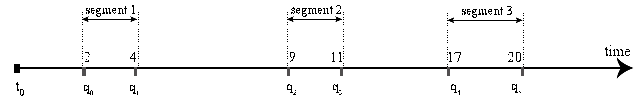
\includegraphics[width=\textwidth]{figs/example_recursive_s.pdf}
	\caption{Segmentation of queries on the timeline for Example \ref{}}
	\label{fig:example_recursive_segmentation}
\end{figure}


\subsection{Dynamic programming approach to find optimal segmentation of the timeline}

Dynamic programming improves the time complexity of finding optimal segmentations in recursive algorithm by utilizing memoization technique \cite{johnsonbaugh2003algorithms}. In the memoization technique, if the cost of a segmentation is calculated, it is stored in a table where the recursive calls can look up the results in the table instead of recalculating them. We can build a table $\mathbf{OPT}$ as a two dimensional array
indexed by $(i, k)$ where $i\in [1, n]$ and $k\in [1, m]$.  Each entry
in the table $\mathbf{OPT}[i,k] = \mathrm{opt}(Q[1,i], k)$.
We can compute $\mathbf{OPT}[i,k]$ in a bottom up fashion \cite{kossmann2000iterative}.

\begin{algorithm}[H]
\SetAlgoLined
\caption{Dynamic programming method to compute $m$ number of optimal segmentations}
\label{alg:dynamic_programming}
\DontPrintSemicolon
 \SetKwFunction{FMain}{computeOPT}
 \SetKwProg{Fn}{Function}{:}{}
 \Fn{\FMain{$Q$, $m$}}{
    $n = |Q|$\;
    \textbf{OPT}$[i,0]$ = $\infty$ \;
    \For{$k \gets 1$ \KwTo $m$}{
    	\For{$i \gets 1$ \KwTo $n$}{
    		$j^* = \underset{j\in[1,i]}{\mathrm{argmin}}(\mathrm{cost}(\mathbf{OPT}[j,k-1]) + \mathrm{cost}(Q[j+1, n]))$ \;
    		$\mathbf{OPT}[i,k] = \mathbf{OPT}[j^*, k-1] \cup \{\mathrm{median}(Q[j+1], n)\}$ 
    	}
    }
}
 
\end{algorithm}

The complexity of computing all the entries of $\mathbf{OPT}$ is $\mathcal{O}(mn^2)$.

\begin{example}
	Given a set of queries $Q={q_0=2,q_1=4,q_2=9,q_3=11}$, we want to compute 3 segmentations from these queries, such that putting a snapshot in each segmentation, make the overall cost of answering to the queries optimal. The process of computing optimal snapshots has been showin Table \ref{table:dynamic_programming}. This method is more efficient than recursive algorithm as for example in the memoization table T[3][2], the recursive call uses the cost stored in T[2][1], T[2][2] and T[2][3] without the need to recalulate them. In this example, the most optimal overall cost is 2 which is achieved by either $\{segment1 =[q_0,q_1],segment2=[q_2],segment3=[q_3]\}$ or $\{segment1 =[q_0], segment2 = [q_1], segment3 = [q_2, q_3]\}$
\label{example:dynamic_programming}
\end{example}

\begin{table}[]
\scriptsize
\renewcommand{\arraystretch}{2}
\setlength\tabcolsep{1pt}
\caption{Memoization table T for dynamic programming approach to compute 3 optimal segmentations from 4 queries.}
\label{table:dynamic_programming}
\begin{tabular}{|l|l|l|l|l|}
\hline
0 & 0 & 0 & 0 & 0 \\ \hline

0 & $T{[}0{]}{[}0{]}+cost(q_0)$& 
$T{[}0{]}{[}1{]}+cost(q_0,q_1) $ & 
$T{[}0{]}{[}2{]}+cost(q_0,q_1,q_2)$&   
$T{[}0{]}{[}3{]}+cost(q_0,q_1,q_2,q_3) $ \\ 
 & $0+0 = 0$ & $0+2 = 2$ & $0+7=7$ & $0+14 = 14$ \\ \hline

0 & 
$T[1][0]+cost[q_0]$ & 
$min\left\{\begin{array}{ll}T[1][1]+cost[q_1] \\ T[1][2]+cost[]\end{array}\right.$&
$min\left\{\begin{array}{lll}T[1][1]+cost[q_1,q_2] \\ T[1][2]+cost[q_2] \\ T[1][3]+cost[] \end{array}\right.$&
$min\left\{\begin{array}{llll}T[1][1]+cost[q_1,q_2,q_3] \\ T[1][2]+cost[q_2,q_3] \\ T[1][3]+cost[q_3] \\ T[1][4]+cost[] \end{array}\right.$\\ 

& $0+0 = 0$ & 
$min\left\{\begin{array}{ll}  0+0 = 0 \\ 0 + 2 = 2 \end{array}\right.$ & 
$min\left\{\begin{array}{lll}  0+5 = 5 \\ 2 + 0 = 2 \\ 7+0=7  \end{array}\right.$ & 
$min\left\{\begin{array}{lll}  0+7 = 7 \\ 2 + 2 = 4 \\ 7+0=7 \\ 14+0 = 14 \end{array}\right.$ \\ \hline

0 & 
$T[2][0]+cost[q_0]$ & 
$min\left\{\begin{array}{ll}T[2][1]+cost[q_1] \\ T[2][2]+cost[]\end{array}\right.$&
$min\left\{\begin{array}{lll}T[2][1]+cost[q_1,q_2] \\ T[2][2]+cost[q_2] \\ T[2][3]+cost[] \end{array}\right.$&
$min\left\{\begin{array}{llll}T[2][1]+cost[q_1,q_2,q_3] \\ T[2][2]+cost[q_2,q_3] \\ T[2][3]+cost[q_3] \\ T[2][4]+cost[] \end{array}\right.$\\ 

& $0+0 = 0$ & 
$min\left\{\begin{array}{ll}  0+0 = 0 \\ 0 + 0 = 0 \end{array}\right.$ & 
$min\left\{\begin{array}{lll}  0+5 = 5 \\ 0 + 0 = 0 \\ 2+0=2  \end{array}\right.$ & 
$min\left\{\begin{array}{lll}  0+7 = 7 \\ 0 + 2 = 2 \\ 2+0=2 \\ 4+0 = 4 \end{array}\right.$ \\ \hline

\end{tabular}
\end{table}


\subsection{Heuristic snapshot placements}
In the heuristic technique, the optimal solution to a problem is not guaranteed however because of the low computational cost and satisfactory results, this approach is used when non-heuristic techniques are inefficient to implement. For the purpose of finding the optimal segmentation of queries for optimal query answering, we utilized K-means clustering technique.

\begin{prop} 
	Given $T_q^* = \{q_0,q_1,...,q_n\}$ as $n$ number of queries performed on the temporal relation $r^T$, we would like to group the $q_i \in T_q^*$ into $m$ number of \textit{"clusters"}. 
\label{prop:heuristic_method}
\end{prop}
Applying K-means clustering methodology to this problem requires to minimize the objective function defined as:
$$J = \sum_{j=1}^{m} \sum_{i=1}^{n} ||q_i^{(j)}-\mu_j||^2$$
where $\mu_j$ is the centroid of $j^{th}$ cluster and $||q_i^{(j)}-\mu_j||^2$ is the squared error function which indicates the distance between each query and their assigned centroids.
Minimizing objective function is achieved by the relocation of $\mu_j$ until no changes occur in the objective function.

\begin{algorithm}[H]
\SetAlgoLined
\caption{K-means clustering to compute $m$ number of segmentations}
\label{alg:Kmeans}
\DontPrintSemicolon
 \SetKwFunction{FMain}{K-Means}
 \SetKwProg{Fn}{Function}{:}{}
 \Fn{\FMain{$T_q^*\{q_1,...,q_n\}$, $m$}}{
    $\{\mu_1,...,\mu_m\} \gets SelectRandomSeeds(\{q_i\in T_q^*\},m)$ \;
	\For{$i \gets 1$ \KwTo $n$}{
		$J \gets argmin_{J^*}||\mu_{J^*}-q_i||^2$ \;
		$\mathcal{L}_j \gets \mathcal{L}_j \cup \{q_i\}$ 
	}
	\For{$j \gets 1$ \KwTo $m$}{
		$\mu_j \gets \frac{1}{\mathcal{L}_j} \sum_{q \in \mathcal{L}_j} q $
	}
	\Return\{$\mu_1,...,\mu_m$\}
}
\end{algorithm}

\section{Blockchain}
In this section we extensively talk about the implementation of a Blockchain based mechanism to verify the trustworthiness of the records. In the first step we talk about temporal tables with security information and then we discuss about the procedure of creating a chain of the records in these tables. In the next steps we talk about steps and rules that needs to be applied in order to verify the trustworthiness of the records in a table, as well as utilizing this mechanism in the case of snapshot materialization.

\subsection{Temporal table with security information}
Let $r_i^T$ be the temporal relational table with attributes $attr(r_i^T)$=$\{attr(r_i), updated,deleted\}$, denote $\alpha_u$ as the security information of the user $u$, including the user's cryptographic keys $<K_{priv}^u, K_{pub}^u>$.


\begin{defn}[digital signature of the transactions] 
	Given a set of records $rec_j =\{rec_1,rec_2,...,rec_n\} \in r_i^T$, the signature of each record could be computed as $$signature(rec_j|\alpha_u)= encrypt(hash(rec_j),K_{priv}^u)$$  
\label{defn:digital_signature}
\end{defn}

Digital signatures provide a strong mean to identify whether or not a record has been submitted by a ligitimate user. They are also used to certify if the record has not been altered as any minor change in the record results in a completely different digital signature. Also faking a digital signature is computationally infeasable, therefore digital signatures provide a strong security guarantees \cite{katz2010digital}.

\begin{defn}[Temporal table with chained security information]
	The temporal relational table with chained security information $r_i^{T*}$ is a table with the attributes $$attr(r_i^{T*}) = attr(r_i^T) \cup \{username,currentSignature, previousSignature)\}$$ where $username$ is the username of the user $u$ who submitted the transaction, $currentSignature = signature(rec_j)$ is the digital signature of the submitted transaction $rec_j$ by $u$ and $previousSignature = rec_{j-1}[currentSignature]$ is the signature of the previous record stored in $r_i^T$. 
\label{defn:temporal_blockchain}
\end{defn}

We are interested in stroring the username of the user who submitted the transaction because it enables us to fetch the public key of the user and verify their digital signature on the submitted record.

\begin{defn}[Chain verification]
	To verify if a chain of the records are valid, the following steps are proposed:
	\begin{itemize}
		\item \textbf{step 1.} verify the $currentSignature$ of individual records.
		\item \textbf{step 2.} check if $rec_j[previousSignature] == rec_{j-1}[currentSignature]$ except for $rec_0$
	\end{itemize}
\label{chain_verification}
\end{defn}
A chain is said to be broken if inconsistent information being gained in any of the above steps.

\begin{example} 
	The Table \ref{temporal_blockchain_table} is an example of a temporal relational table with chained security information. With assumption that each record is a block, this table also could be depicted as Figure \ref{fig:blockchain_representation} which is the blockchian representation of Table \ref{temporal_blockchain_table}.
\label{example:blockchain}
\end{example}

\begin{center}
\begin{table}
	\centering
	\footnotesize
	\caption{Temporal Table $r_1^T$ with chained security information}
	\label{temporal_blockchain_table}
	\begin{tabular}{p{0.5cm}p{0.5cm}p{1cm}p{0.5cm}p{1.7cm}p{1.7cm}p{1.5cm}p{1.5cm}p{1.5cm}}
		\hline
		r\_id & id & item      & value  & updated  & deleted & username & curSgn & prevSgn \\ \hline
		151& 21 & Ruler    & 3.25  & 2018-02-10  &  - & Bob &r3T49TR & 0\\  
		152& 21 & Ruler    & 3.25  & -  &  2018-02-20 & Alice & yu0PmER & r3T49TR\\
		153& 22 & Pencil    & 8.0  & 2018-03-21  &  - & Alice & gI90vjN & yu0PmER\\
		154& 23 & Pen    & 12.0  & 2018-03-30  &  - & Bob & 89Ec578 & gI90vjN\\
		155& 22 & Pencil & 7.50  & 2018-04-01 & - & Eve & Ipu32h6 & 89Ec578\\ \hline
	\end{tabular}
\end{table} 
\end{center}

\begin{figure}
	\centering
	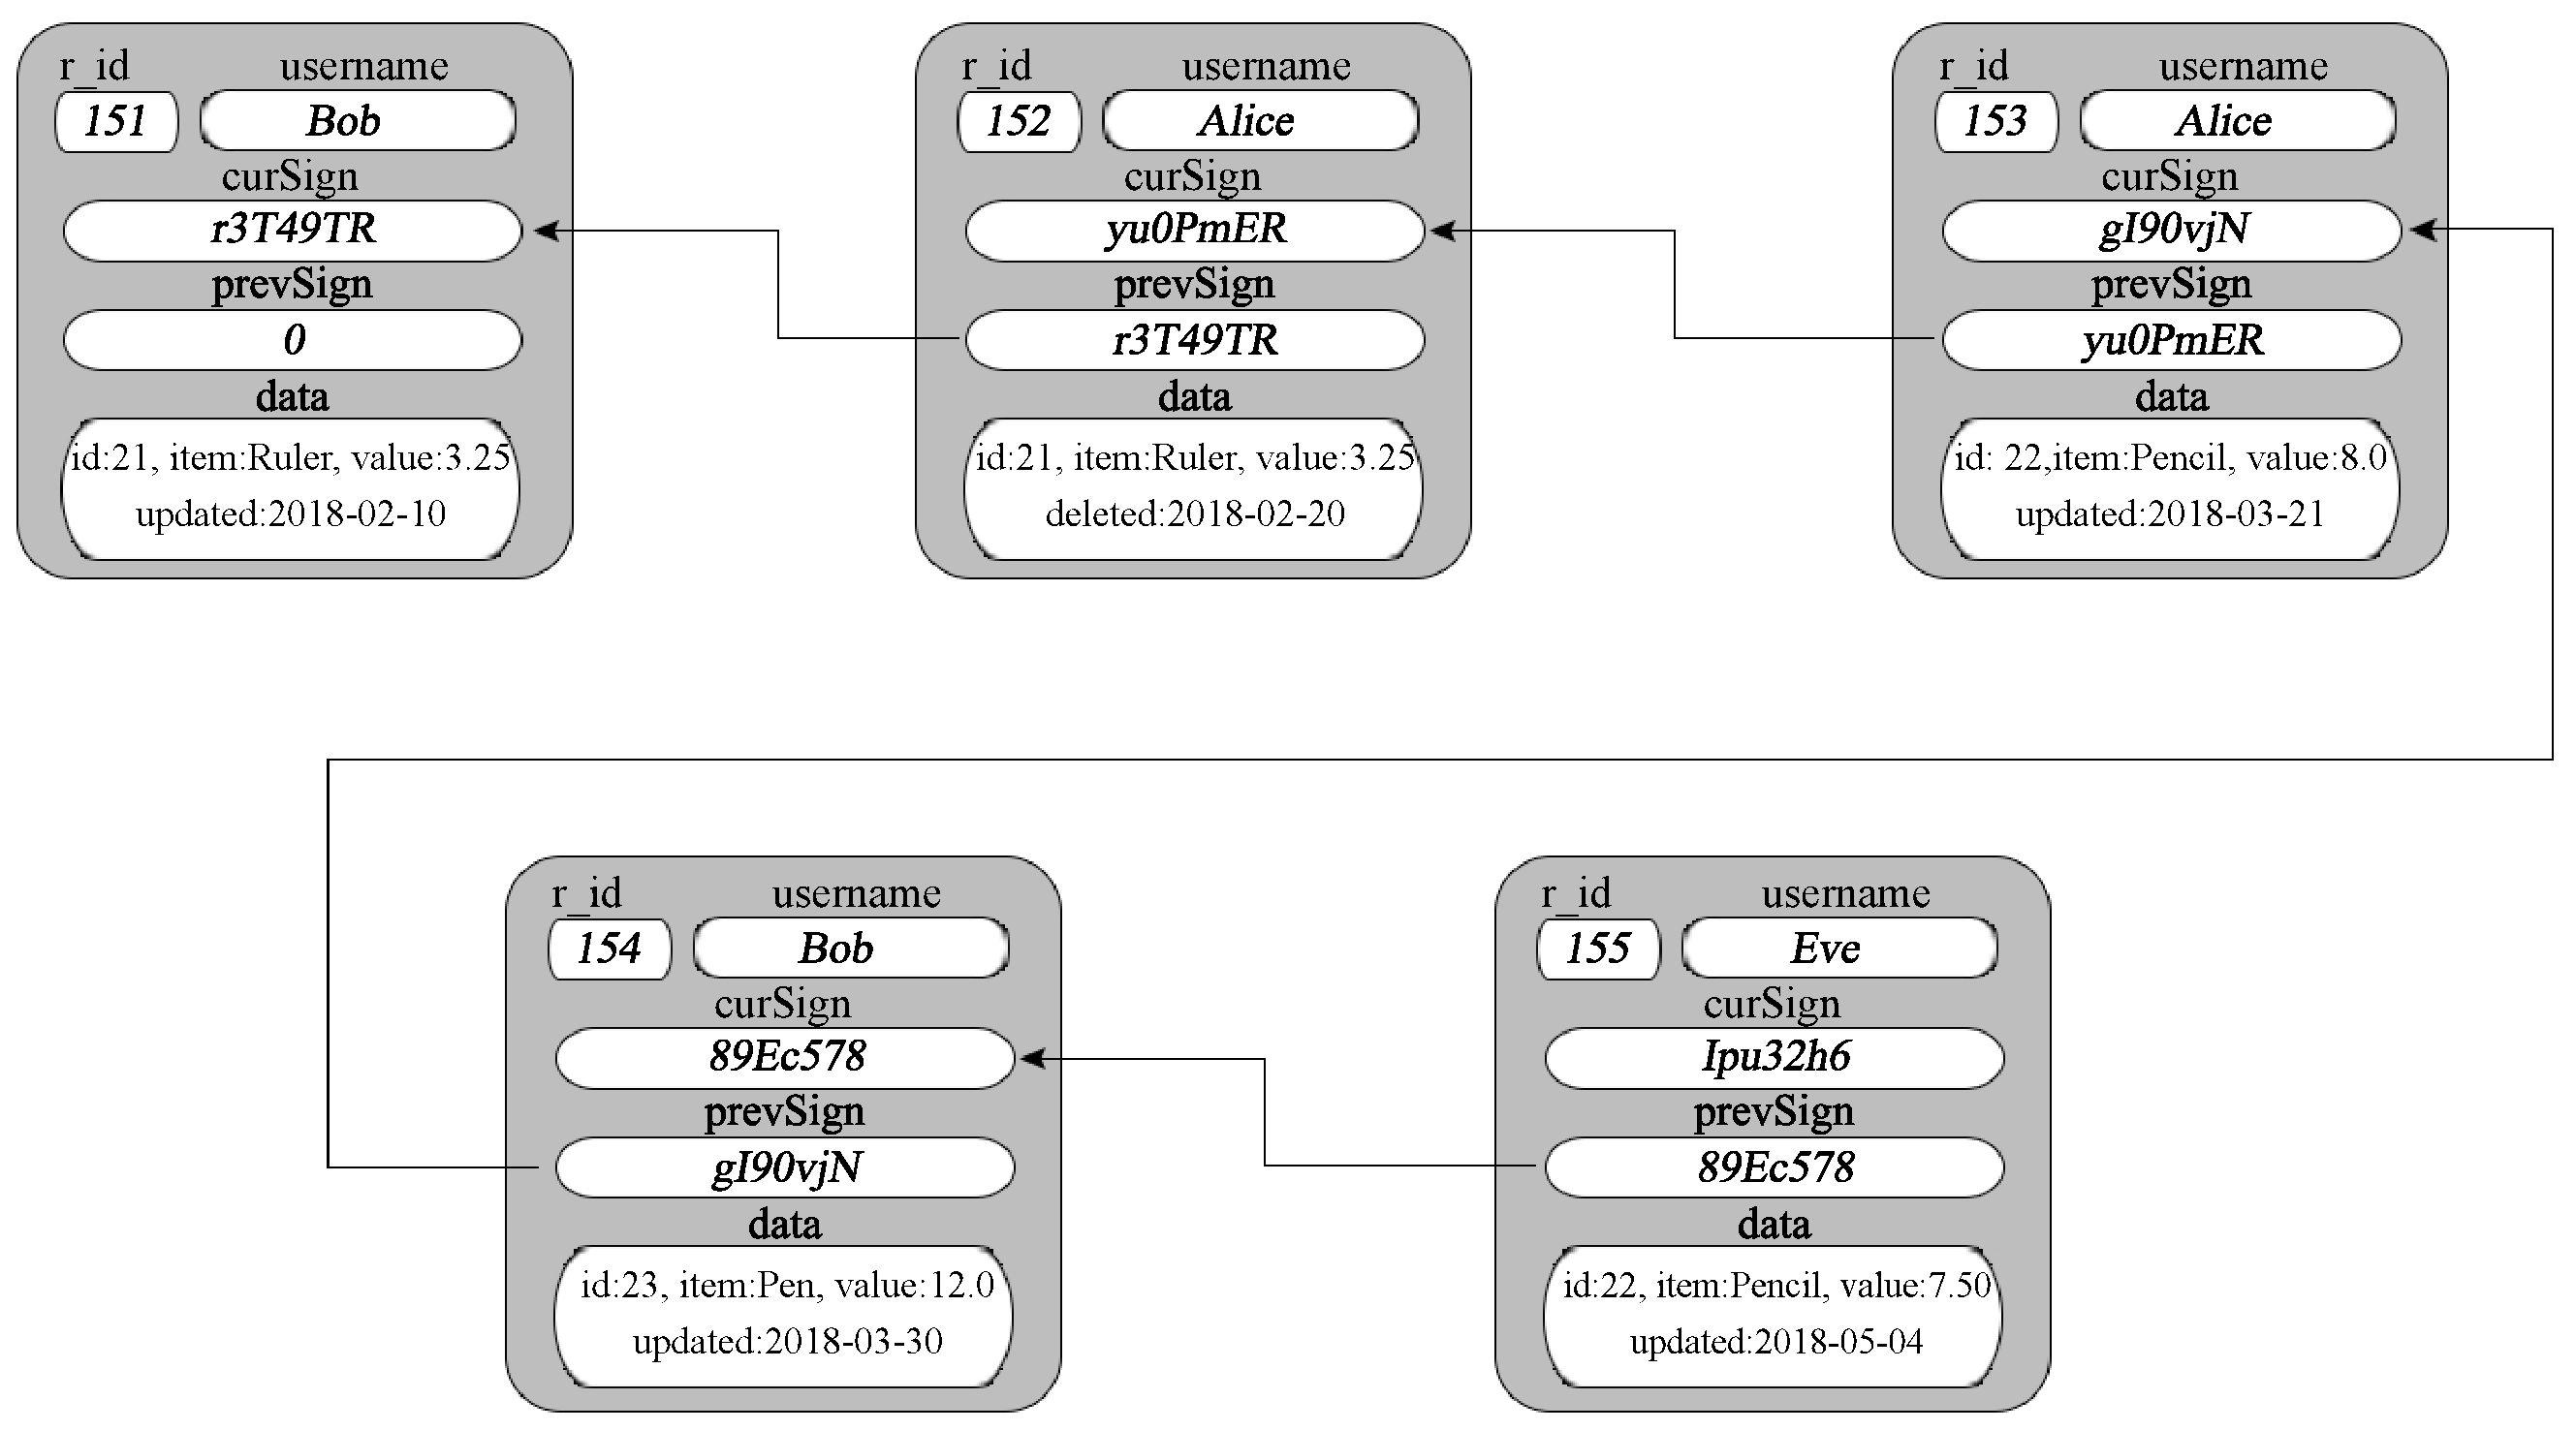
\includegraphics[width=\textwidth]{figs/temporal_blockchain.pdf}
	\caption{Blockchain representation of the table $r_1^T$.}
	\label{fig:blockchain_representation}
\end{figure}

\subsection{Trusted Snspshots}
Using blockchain to ensure the trustworthiness of data, requires a consistent chain of blocks. To make sure that a chain is consistent, all the blocks in the temporal table need to be visited and their trustworthiness need to be examined. This computation requires linear time and makes application of snapshot materialization that we discussed earlier pointless. To solve this problem, we propose the idea of trusted snapshots.

\begin{defn}[Trusted Snapshots] 
	The trusted snapshot $s^*$ is a table with attributes $attr(s)\cup \{signature\}$ where $$tail(s^*[signature]) = signature(\sum_{i=0}^n (rec_i):rec_i \in s)$$
\label{defn:trusted_snapshot}
\end{defn}

\begin{defn}[Trusted snaphsot materialization] 
	We earlier talked about the materialization of snapshots for the sake of less computational time when querying the temporal database. To ensure the trustworthiness of the records while materializing trusted snapshots, we propose the following steps to be taken:
	\begin{itemize}
		\item \textbf{step 1.} the signature of the materialized snapshot to be checked.
		\item \textbf{step 2.} The trustworthiness of the records which fall in between the query $q$ and snapshot $s$ to be verified using blockchain verification.
	\end{itemize}
	The steps which should be taken to verify the trustworthiness of the records in the case of snapshot materialization could be depicted as Figure \ref{fig:blockchain_snapshot_materialization}.
\label{defn:trusted_snapshot}
\end{defn}
\begin{figure}
	\centering
	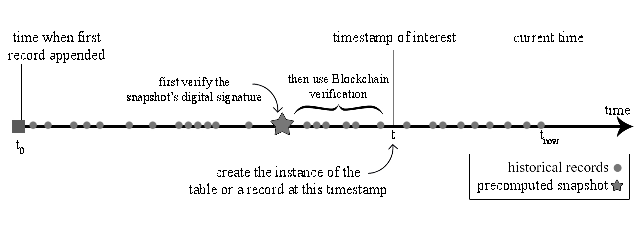
\includegraphics[width=\textwidth]{figs/trusted_snapshot_materialization.pdf}
	\caption{verify trustworthiness of the records in snapshot materialization}
	\label{fig:blockchain_snapshot_materialization}
\end{figure}

The remaining issue is that, to digitally sign the records in $s$, we need to make sure the trustworthiness of the records before hand, therefore we propose the following rules for that purpose:

\begin{itemize}
	\item The first snapshot's records trustworthiness is checked using blockchain verification.
	\item The subsequent snapshots materialize their previous snapshot, hence we take the same steps that was proposed in Proposition \ref{}
\end{itemize}

Figure \ref{fig:signing_snapshots} depicts the rules that needs to be followed when signing a precomputed snapshot.

\begin{figure}
	\centering
	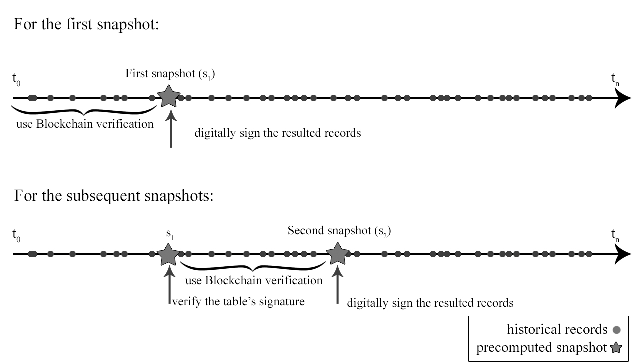
\includegraphics[width=\textwidth]{figs/signing_snapshots.pdf}
	\caption{rules that needs to be followed when signing precomputed snapshots}
	\label{fig:signing_snapshots}
\end{figure}

\section{Discussion}
In this section, the problem of linear time for query answering in append-only databases discussed. Creating snapshots and looking for the form of a table in an specific time on append-ony databases are inefficient therefore we proposed to place $m$ number of snapshots for materialization of subsequent queries. these snapshots indicate the latest version of a database until that specific time. Although it seems to be inefficient to store $m$ number of snapshots in a system, but with current cloud storages, it doesnot seem to be an overly burden task anymore. Note that $m$ is determined by checking the available resources of the host system.

In the first step, we stored the timestamp of the previous queries on the database to have the patterns of the queries on the timeline. Pattern of the queries ables us to identify the hotspots on the timeline. We argue that it is highly likeley that the the subsequent queries to be performed in these hotspots, therefore we proposed to group the queries on the hotspots and allocate one snapshot for each group for materialization. However the question which needed to be answered was to find $m$ number of optimal segmentations of queries which reduce the overall cost of answering to the queries on the temporal append-only database.

To find $m$ number of optimal segmentation, we first solved the problem of finding an optimal position to place a single snapshot. We proved that the optimal place for a single snapshot is the median of the queries, hence if $m$ number of segmentations were created, the optimal position to place snapshot within each segmentation is the median of the segmentation queries. To find the optimal segmentations we utilized three different methods : recursive algorithm, dynamic programming and K-Means clustering. Each method has their pros and cons which are shown in Table \ref{table:segmentation_comparison}. In the next section we support the comparison between methods with different experiments and we depict the observations followed by drawing a conclusion. 

\begin{center}
\begin{table}
	\centering
	\small
	\caption{Snapshot $s_2$ at $t = 2018-03-15$}
	\label{table:segmentation_comparison}
	\begin{tabular}{p{4cm}p{4cm}p{4cm}}
		\hline
		method & Pros  & Cons  \\ \hline
		Recursive algorithm & Exact optimal solution & computationally expensive for large number of queries and segmentations   \\ \hline
		Dynamic programming & Exact optimal solution & computationally expensive for large number of queries and segmentations\\ 
		  & Computationally cheaper than dynamic programming &    \\ \hline
		K-Means clustering & Fast in computation & optimal solution not guaranteed \\ \hline
	\end{tabular}
\end{table}
\end{center}

\chapter{System Implementation And Experimental Evaluation} \label{chap:system_implementation}
    This chapter attempts to discusses the experiments performed to evaluate the proposed solutions as well as the tools that were utilized for the implementation of the system. Section \ref{sec:experimental_setup} provides information about the system design, choice of software and programming languages that were utilized to develop the system. Section \ref{sec:evaluation_of_snapshot_materialization} provides an evaluation of discussed methods for snapshot materialization by setting up different experiments. In section \ref{}, different malicious activity scenarios on the relational database are introduced and the Blockchain solution to identify these activities is discussed.

	\section{Development environment and application development tools} \label{sec:development environment}
		To setup the development environment of the project, we used the 'Leda' research server provided by the department of scinece at the University of Ontario Institute of Technology with the ubuntu 16.04 operating system installed. The application could be developed by various tools, but since one important goal of this project was to be able to generalize our proposed solution for different systems, we needed to choose the tools that are popular among the developers for the development of their system. For the database choice, we favored the use of postgreSQL simply because of its wide adoptation by the industry \cite{cook2017docker}. 

		The experiments scripts were mainly developed by using Python 2.7 programming language. We started off by generating database using the TPCH schema with 1,000,000 tuples in the main table. We also generated a synthetic temporal database by performing a set of random record modification, insertion and deletion updates at 1000 distinct timestamps. This created a temporal table with 1,000 timestamps. To be able to manage the relational database and perform queries on the tables, we utilized SQL query language.

		Generation of snapshots using the records stored in the temporal tables required time series analysis and performing numbers of aggregations and self-joins on the table. In order to make this process more efficient and less cumbersome, we utilized the windowing function that is part of the SQL standard and is supported by the relational databases \cite{leis2015efficient}.

		To evaluate the effectiveness of snapshot materialization, the optimal snapshot placement had to be examined in different query distributions on the timeline. The Python's Numpy library gave us the ability to simulate some hotspots on the timeline and distribute the queries on the timeline with various distribution models. After running the snapshot materialization experiments and collecting data, we utilized the Python's plotly library in order to visualize the collected data.

		Cryptography is the method that Blockchain utilizes to secure data that are stored in it and link the blocks of data together. For the purpose of creating a Blockchain of the records, we used the Python's pycrypto 2.6.1 library \footnote{https://pypi.org/project/pycrypto/}. The pycripto package contains various encryption algorithms and hash functions as well as a built-in function to create digital signatures that makes it suitable for the creation of the Blockchain.

	\section{Evaluating snapshot materialization} \label{sec:evaluation_of_snapshot_materialization}
		In this section we discuss the evaluation of snapshot materialization through different experiments. We start off by showing a method to create snapshots using the data that are stored in the temporal database. Then we show the problem of linear computational time in performing queries on a temporal relational table and we evaluate the placement of a single snapshot for matrialization in different timestamps. In the next step we show the effectiveness of utilizing multiple number of precomputed snapshots for materialization and at the end, the various approaches discussed in section \ref{sec:optimal_multiple_snapshot} to place multiple snapshots on the timeline are put to an experiment and their performance is evaluated.

		\subsection {Generating snapshots by using records in a temporal database} \label{sec:snapshot_generation}
			We can construct the snapshots using simple windowing functions (as in supported by PostgreSQL \cite{momjian2001postgresql}).
    		\vspace{1em}
			\begin{center}
				\begin{table}[b]
					\centering
					\small
						\begin{tabular}{|l|} \hline
							$\mathrm{snapshot}(r, t)$ = \\
							\verb|| \textsc{With} $T$ \textsc{as} ( \\
							\verb|   | \textsc{select} id, $\{\mathrm{last\_value}(x) \mathrm{\ as\ } x:
							x\in attr(r)\}$ \textsc{over} $W$ \\
							\verb|   | \textsc{from} $r^T$ \\
							\verb|   | \textsc{where} updates $\leq t$ \\
							\verb|   | \textsc{window} $W$ \textsc{as} 
							\textsc{partition by} id \textsc{order by} updates\\
							\verb|| ) \\
							\verb|| \textsc{select} id, $\{x: x\in attr(r)\}$ \textsc{from} $T$ \\
							\verb|| \textsc{where not} $T.$deleted \\ \hline
						\end{tabular}
					
				\end{table}
			\end{center}
			The query $\mathrm{snapshot}(r, t)$ computes the snapshot of $r$ at timestamp $t$ by applying the latest update of each tuple up to timestamp $t$, while removing tuples that have been deleted.

		\subsection{Evaluating the linearity of the queries on a temporal table} \label{sec:evaluating_linearity}
			As discussed in proposition \ref{prop:linear_time}, preforming queires to create snapshots in a timestamp of interest from the historical data, require visiting all the records before that timestamp and apply all the updates on the table. Over time, when the temporal tables grow in size, performing such computations may become expensive and inefficient. To prove it experimentally, we implemented a function to perform snapshot creation query on our temporal table and record the query runtime. Then we performed this query 100 times while sliding the timestamp of the query on the timeline of the temporal table. By sliding the timestamp, in each iteration of the query, more records needed to be visited and more updates needed to be applied. From the runtime records the costline was created which is shown if Figure \ref{fig:linear_time}. 

			Figure \ref{fig:linear_time} clearly proves our claim that computation of snapshots on a temporal table requires linear time. The issue of linearity in computation of snapshots makes such tasks on a very large table inefficient. For example in this experiment, the computational cost of 100th query is significantly more expensive than computational cost of 20th query, due to the number of queries which were needed to be visited.

			\begin{figure}
				\centering
				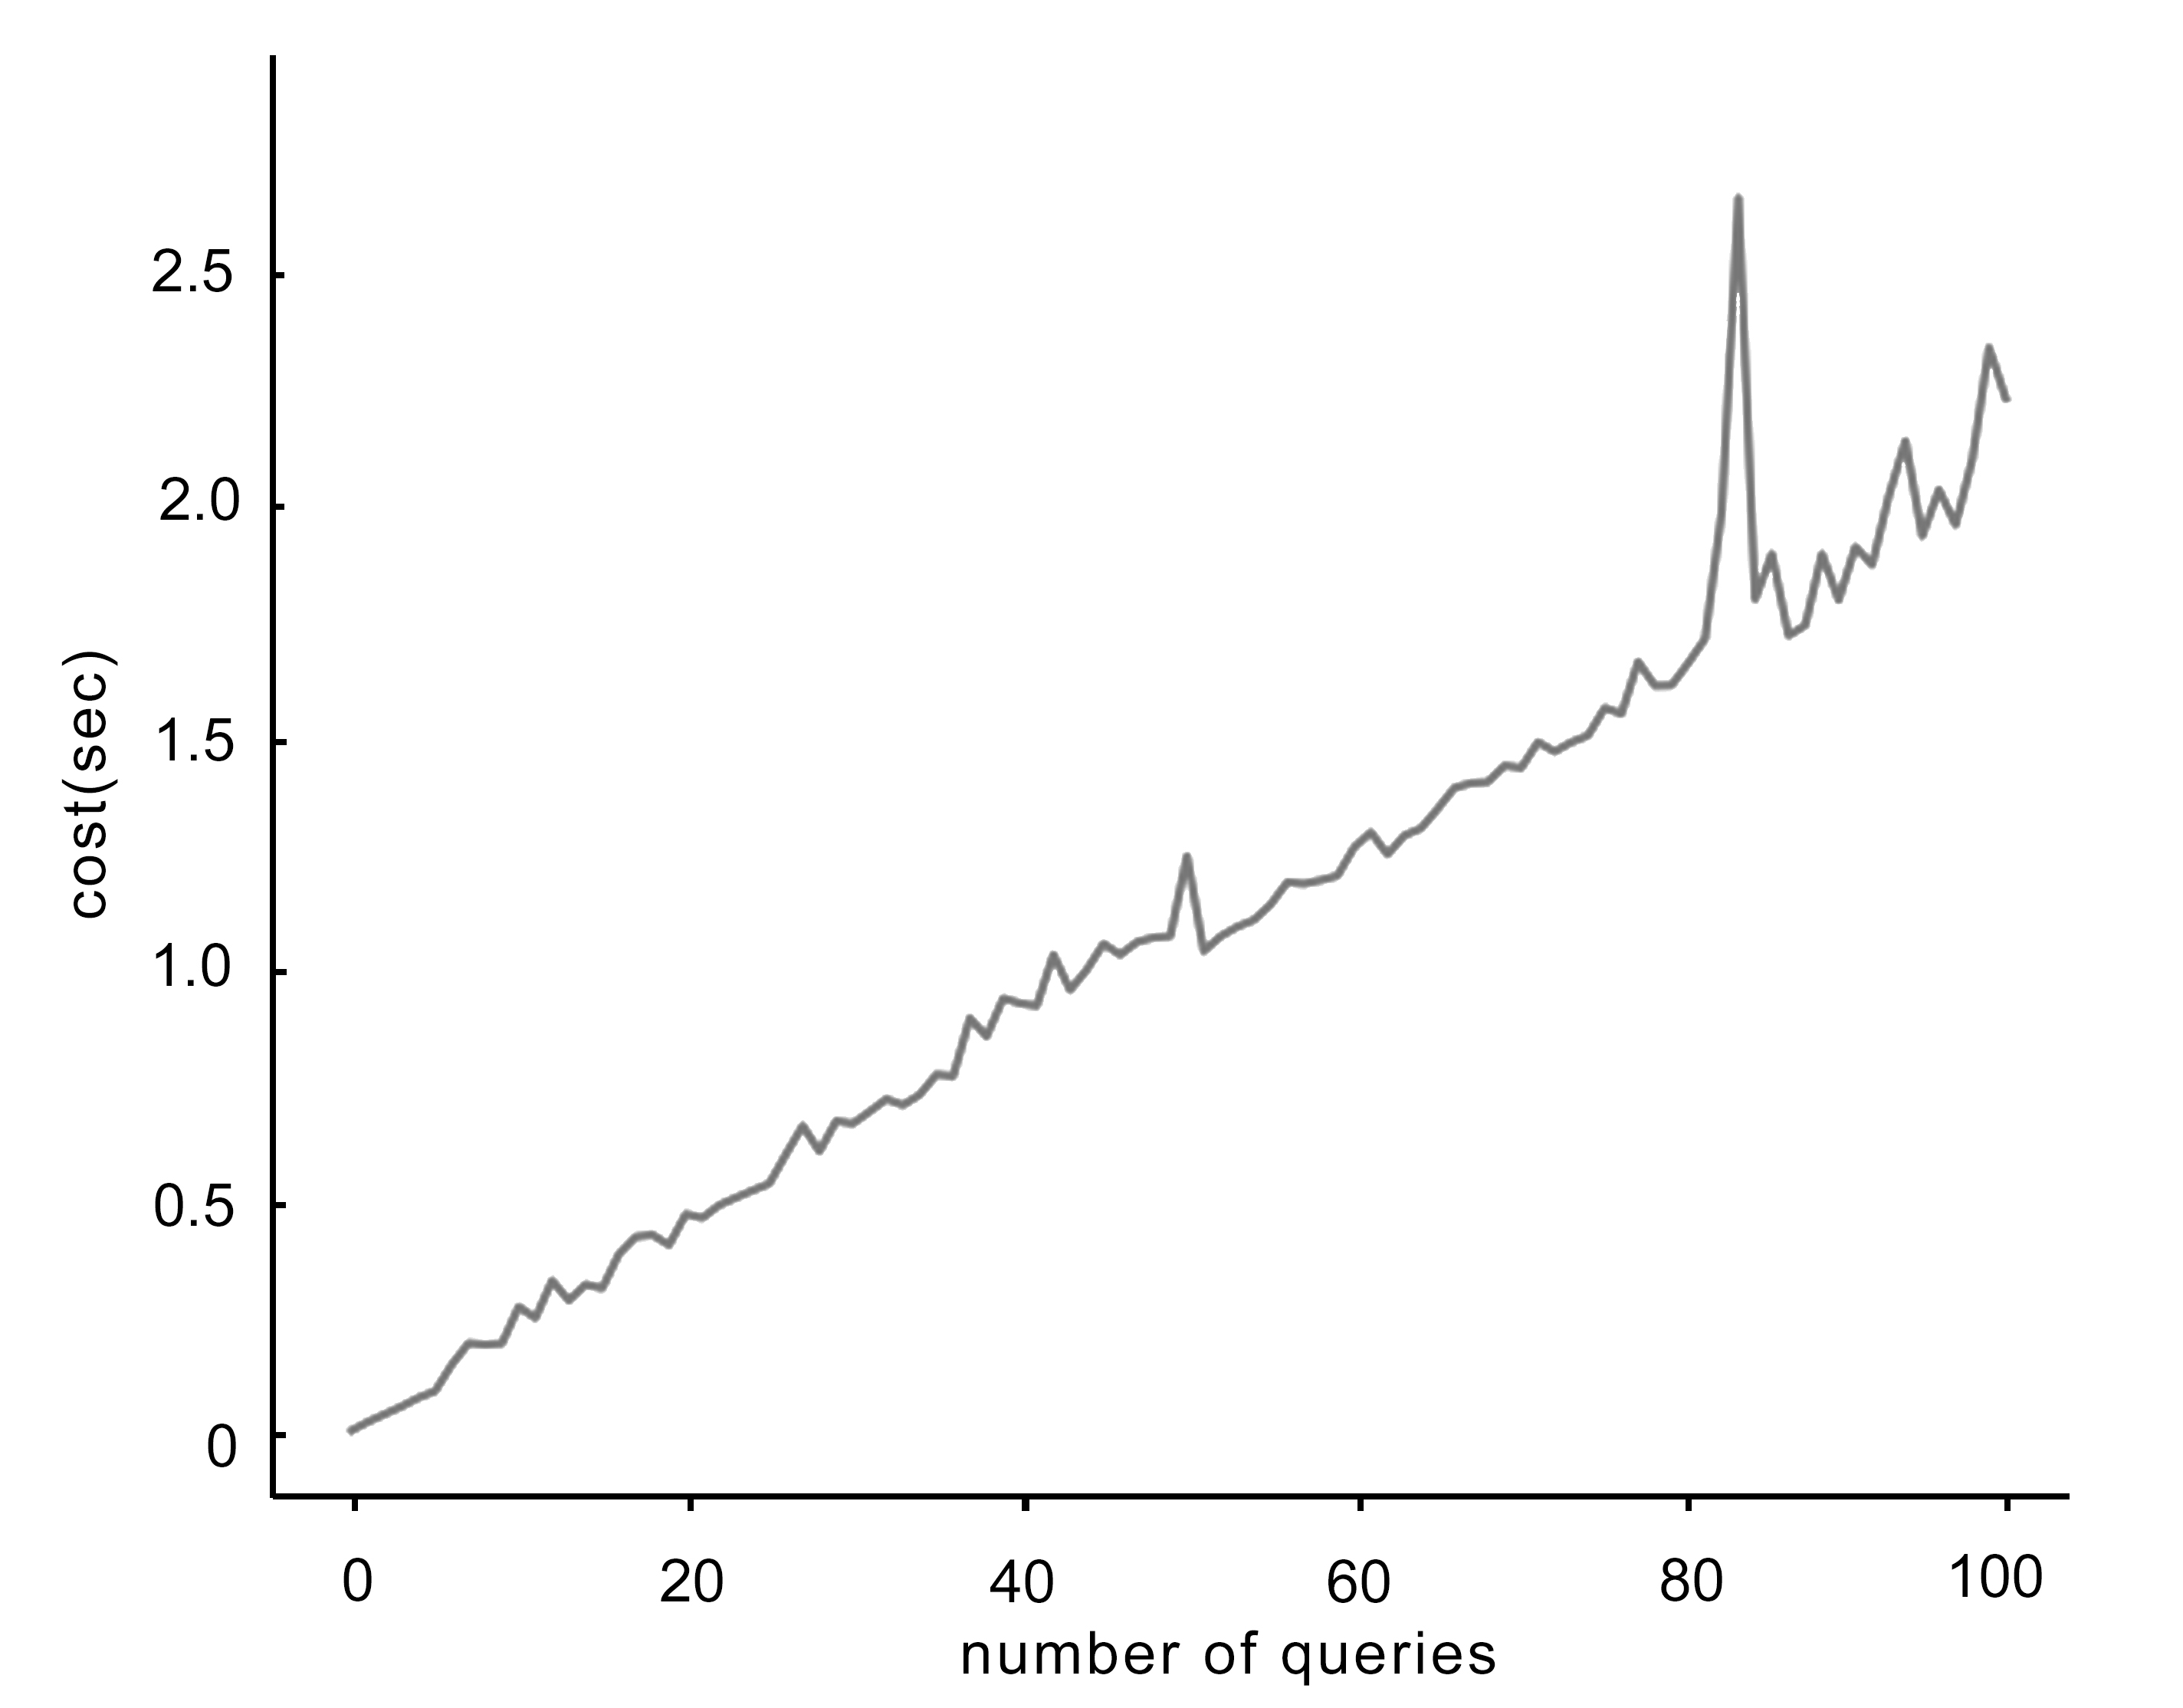
\includegraphics[width=120mm]{figs/runtime.jpg}
				\caption{Linear time in computation of snapshots without snapshot materialization}
				\label{fig:linear_time}
			\end{figure} 

		\subsection{Evaluating materialization of a single snapshot} \label{sec:evaluating_single_snapshot}
			To illusterate the the optimal position on the timeline to place a single snapshot for materialization, we sampled 60 query timestamps from our temporal database and randomly placed 60 number of queries on its timeline. In the next step we placed a single snapshot that each query materialized to perform the task and recorded the overal cost of queries on that timeline using definition \ref{defn:cost_of_query_answering}. To see how the position of materialized snapshot may affect the overal cost of query answering, we slided the timestamp of the snashot on the timeline and recorded the overal cost in each snapshot timestamp. The resulted cost line obtained from sliding the snapshot is depicted in Figure \ref{fig:single_snapshot}. 

			The resulted cost line shown in Figure \ref{fig:single_snapshot} clearly shows that the position of a snapshot directly affects the overal cost of query answering on the temporal table. In proposition \ref{prop:compute-median} we mathematically proved that the median of the queries is the optimal position for snapshot materialization. Therefore in this experiment we calculated the median of the queries which is shown with a red circle in figure \ref{fig:single_snapshot}. As it could be seen, the median of the queries is exactly located in a position where the cost line curve's global minimum is. This illustrates that the median of the queries is the most optimal position to place a single snapshot for materialization.

			\begin{figure}
				\centering
				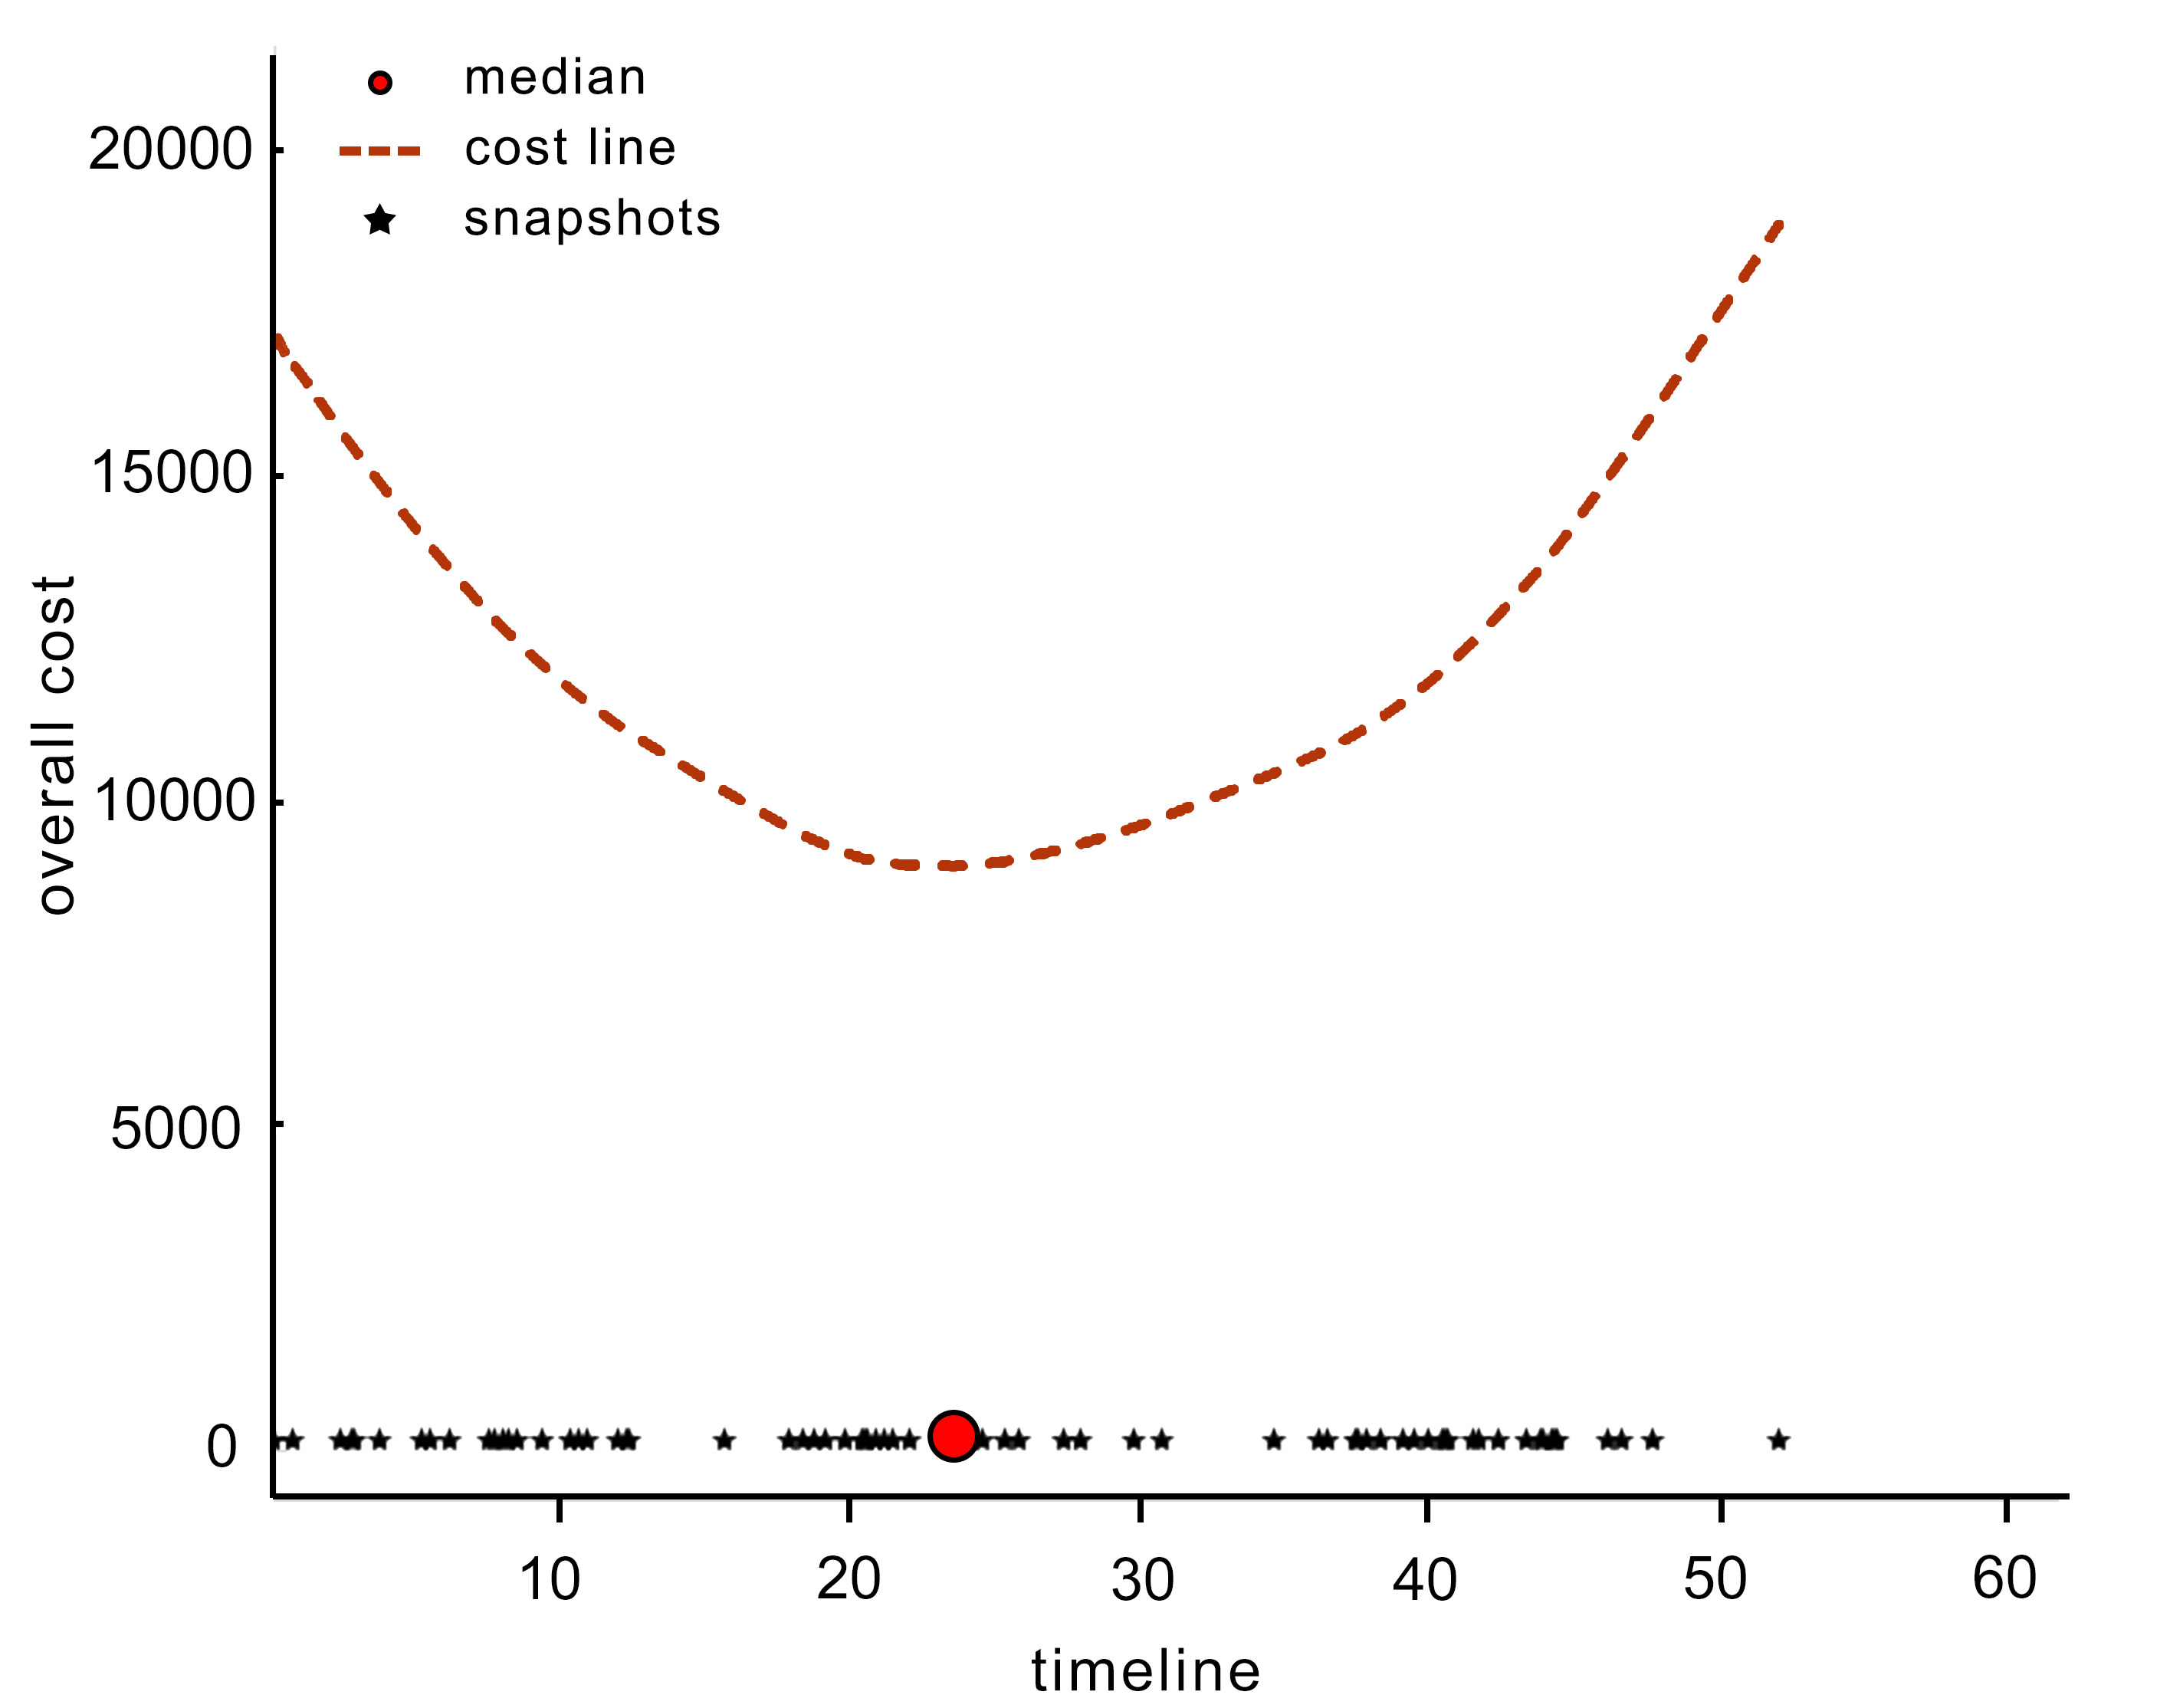
\includegraphics[width=90mm]{figs/single_snapshot.jpg}
				\caption{Cost of query answering using a single snapshot over different snaptshot timestamps}
				\label{fig:single_snapshot}
			\end{figure} 

		\subsection{Evaluating materialization of multiple snapshot} \label{evaluating_multiple_snapshots}
			To evaluate the performance of our optimal snapshot computation, we evaluated the recursive formulation given
			by Section \ref{sec:recursive_algorithm}, the dynamic programming formulation given by Section \ref{sec:dynamic_programming_optimal_segment} and heuristic method given by Section \ref{sec:heuristic_optimal}. 

			To illustrate that the optimal snapshot placement indeed produces the best query answering performance, we compared the query answering cost of three approaches:
			\begin{itemize}
				\item Pick $m$ random timestamps to place the snapshots.
				\item Pick $m$ evenly intervaled timestamps to place the snapshots.
				\item Pick $m$ timestamps computed by dynamic programming.
			\end{itemize}

			\begin{figure}
				\centering
				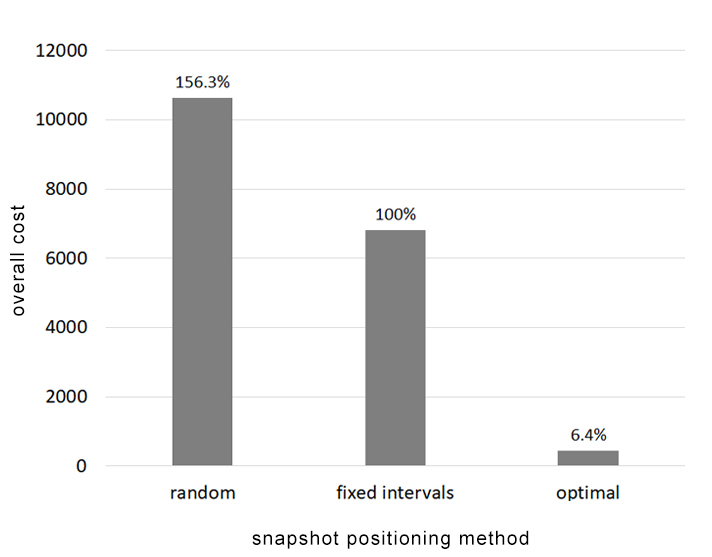
\includegraphics[width=80mm]{figs/various_scenarios_cost.jpg}
				\caption{Query answering cost with forty snapshots with various approaches to place snapshots for materialization}
				\label{fig:approaches_cost}
			\end{figure} 

			Figure \ref{fig:approaches_cost} shows that the placements obtained by dynamic programming clearly beats the other two approaches.

			In order to evaluate the effectiveness of $m$ number of snapshots to lower the overal cost of query answering, we recorded the overal cost of queries in various number of snapshots. Figure \ref{fig:snapshots_cost} shows that as the number of snapshots for materialization increases, the overal cost of answering to the queries drops.

			\begin{figure}
				\centering
				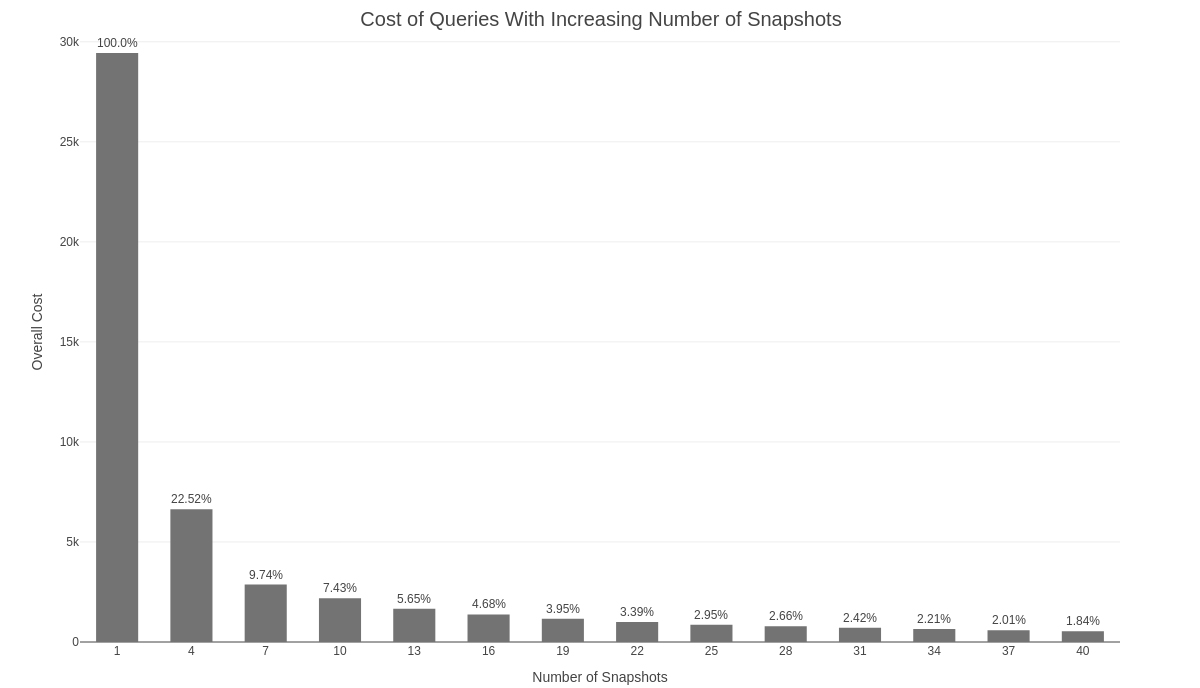
\includegraphics[width=\textwidth]{figs/various_snapshot.jpg}
				\caption{Query answering cost with increasing number of snapshots}
				\label{fig:snapshots_cost}
			\end{figure} 

		\subsection{Implementation of recursive algorithm} \label{sec:recursive_implementation}
			Recursive method was our first approach to find $m$ number of optimal segmentations of the timeline for snapshot placement. The recursive algorithm of this operation is given as Algorithm \ref{alg:recursive}.

			\begin{algorithm}
				\SetAlgoLined
				\caption{Recursive algorithm method to compute $m$ number of optimal segmentations}
				\SetAlCapNameFnt{\tiny}
				\label{alg:recursive}
				\DontPrintSemicolon
				 \SetKwFunction{FMain}{computeOPT}
				 \SetKwProg{Fn}{Function}{:}{}
				 \Fn{\FMain{$Q$, $m$}}{
				    $n = |Q|$\;
				    \textbf{OPT}$[i,0]$ = $\infty$ \;
				    \For{$k \gets 1$ \KwTo $m$}{
				    	\For{$i \gets 1$ \KwTo $n$}{
				    		$j^* = \underset{j\in[1,i]}{\mathrm{argmin}}(\mathrm{cost}(\mathbf{OPT}[j,k-1]) + \mathrm{cost}(Q[j+1, n]))$ \;
				    		$\mathbf{OPT}[i,k] = \mathbf{OPT}[j^*, k-1] \cup \{\mathrm{median}(Q[j+1], n)\}$ 
				    	}
				    }
				}
			\end{algorithm}

		\subsection{Implementation of dynamic programming} \label{sec:dynamic_implementation}
			Dynamic programming was the second approach that we utilized in order to find $m$ number of optimal segmentation of the timeline for snapshot placement. The dynamic programming uses the memoization technique in which the algorithm stores the result of expensive function calls in a table, and retrieve the result from the table, when the same inputs to the function is given. This approach could be implemented using Algorithm \ref{alg:dynamic_programming}.
			\begin{algorithm}
				\SetAlgoLined
				\caption{Dynamic programming method to compute $m$ number of optimal segmentations}
				\SetAlCapNameFnt{\tiny}
				\label{alg:dynamic_programming}
				\DontPrintSemicolon
				 \SetKwFunction{FMain}{computeOPT}
				 \SetKwProg{Fn}{Function}{:}{}
				 \Fn{\FMain{$Q$, $m$}}{
				    $n = |Q|$\;
				    $minVal = \infty$ \;
				    \For{$i \gets 1$ \KwTo $m$}{
				    	\For{$j \gets 1$ \KwTo $n+1$}{
				    		\For{$k \gets 1$ \KwTo $j$}{
				    			$minVal = \mathrm{min}(\textrm{minVal},\mathbf{Table}[i,k] + \mathrm{cost}(Q[j-k:]))$
				    		}
				    	$\mathbf{Table}[i,j] = minVal$
				    	}
				    }
				}
			\end{algorithm}

		\subsection{Implementation of heuristic method} \label{sec:implementation_heuristic}
			To evaluate the performance of heuristic method in finding $m$ number of optimal segmentation of the timeline for snapshot placement, we chose K-means clustering method. Although the K-means clustering method doesnot guarantee the most optimal solution of creating the segmentations, but we expect a satisfactory results obtained from this method.

			The K-means clustering algorithm is given as Algorithm \ref{alg:Kmeans}.
			\begin{algorithm}
				\SetAlgoLined
				\caption{K-means clustering to compute $m$ number of segmentations}
				\label{alg:Kmeans}
				\DontPrintSemicolon
				 \SetKwFunction{FMain}{K-Means}
				 \SetKwProg{Fn}{Function}{:}{}
				 \Fn{\FMain{$T_q^*\{q_1,...,q_n\}$, $m$}}{
				    $\{\mu_1,...,\mu_m\} \gets SelectRandomSeeds(\{q_i\in T_q^*\},m)$ \;
					\For{$i \gets 1$ \KwTo $n$}{
						$J \gets argmin_{J^*}||\mu_{J^*}-q_i||^2$ \;
						$\mathcal{L}_j \gets \mathcal{L}_j \cup \{q_i\}$ 
					}
					\For{$j \gets 1$ \KwTo $m$}{
						$\mu_j \gets \frac{1}{\mathcal{L}_j} \sum_{q \in \mathcal{L}_j} q $
					}
					\Return\{$\mu_1,...,\mu_m$\}
				}
			\end{algorithm}

		\subsection{Evaluating approaches for optimal placement of $m$ snapshots} \label{sec:evaluating_approaches}
			In this research, we examine 3 approaches to find the optimal timestamps for $m$ number of snashots for materialization. The performed approaches are:
			\begin{itemize}
				\item Recursive algorithm.
				\item Dynamic programming.
				\item K-Means clustering.
			\end{itemize}

			In the first experiment of this category, we evaluate the performance of each approach with respect to variable number of snapshots but fixed number of queries. That is, although the goal of the experiment is to find $m$ number of optimal timestamps for snapshots for materialization, but we start $m=1$ and we increase $m$ in each iteration. For this experiment we sampled 140 number of queries and evalueted the runtime of each approach while increasing the number of requested snapshots.

			\begin{figure}
				\centering
				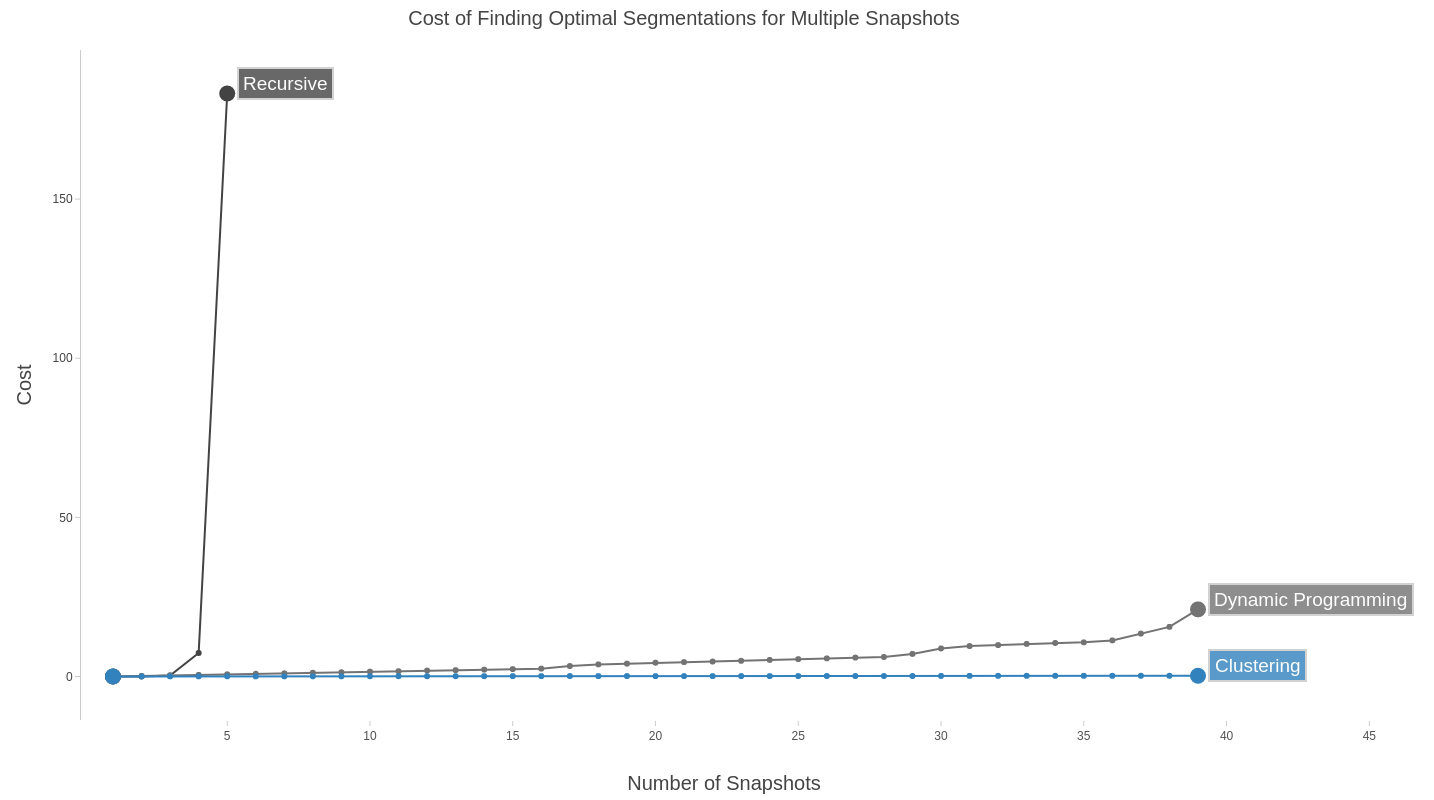
\includegraphics[width=\textwidth]{figs/variable_snapshots.jpg}
				\caption{Optimization time with respect to the number of snapshots}
				\label{fig:variable_snapshots}
			\end{figure} 

			\begin {center}
			\begin{table}
				\centering
				\caption{Optimization time with respect to the number of snapshots}
				\label {table:variable_snapshots}
				\begin{tabular}{p{2cm}p{3cm}p{3cm}p{3cm}}
					\hline
					Snapshots & Recursive      & Dynamic  & Clustering \\ \hline
					1 & 0.0002    & 0.01  & 0.01  \\  
					2 & 0.01    & 0.17  & 0.02  \\
					3 & 0.32    & 0.34  & 0.03  \\
					4 & 7.39 & 0.52  & 0.04  \\
					5 & 183.18 & 0.69  & 0.06 \\
					10 & N/A    & 1.52  & 0.08  \\
					15 & N/A & 2.33  & 0.12  \\ 
					20 & N/A & 4.33  & 0.12  \\ 
					25 & N/A & 5.46  & 0.14  \\ 
					30 & N/A & 8.81  & 0.17  \\
					35 & N/A & 10.74  & 0.21  \\
					40 & N/A & 21.09  & 0.24  \\\hline
				\end{tabular}
			\end{table}
			\end{center}

			Figure \ref{fig:variable_snapshots} and Table \ref{table:variable_snapshots} depict the observations of the experiment. The graph shows that in comparison with dynamic programming and K-means clustering, the recursive algorithm is computationally more expensive such that we couldnot utilize this technique to find more than 5 optimal timestamps for snapshots due to the large computational time. 

			\begin{figure}
				\centering
				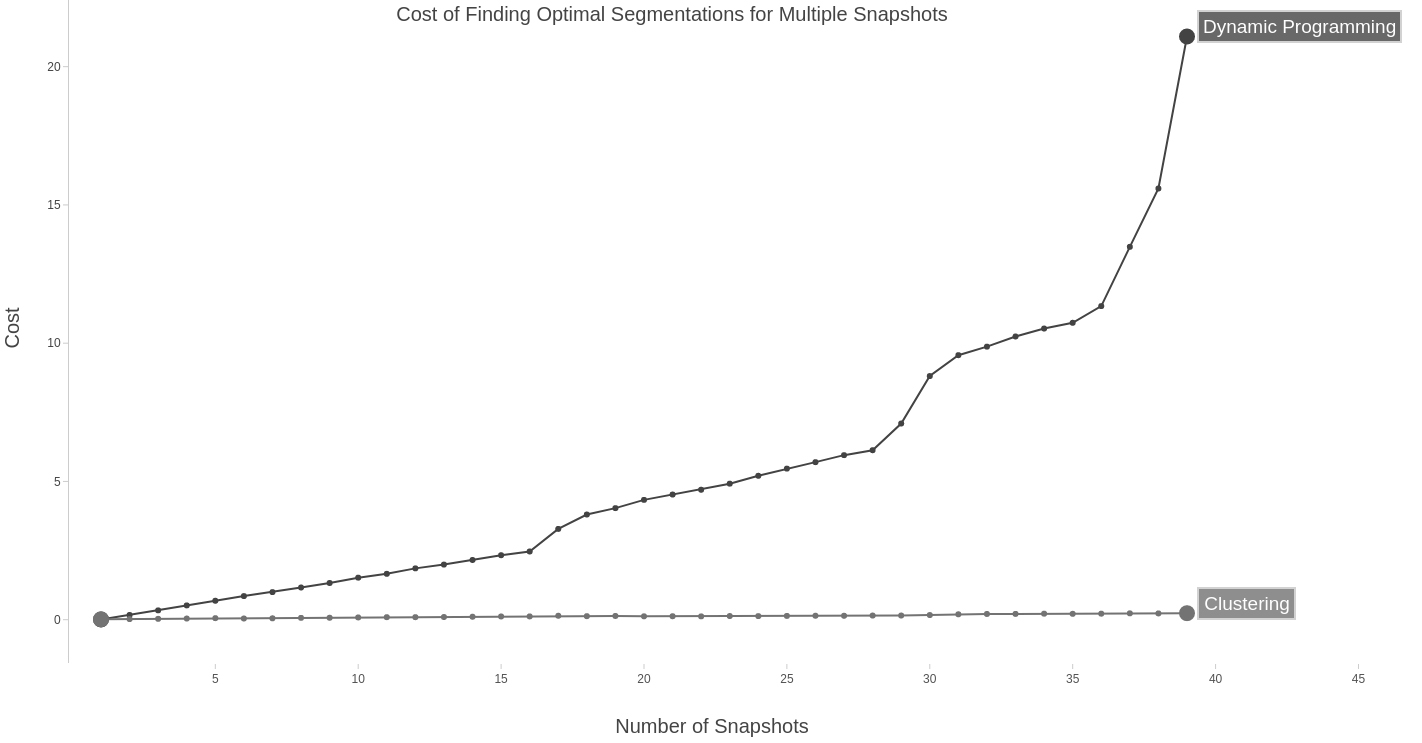
\includegraphics[width=\textwidth]{figs/multiSnapDouble.jpg}
				\caption{Optimization time with respect to the number of snapshots}
				\label{fig:variable_snapshots_2}
			\end{figure} 

			\begin{center}
			\begin{table}
				\centering
				\caption{Optimization time with respect to the number of snapshots}
				\label {table:variable_snapshots_2}
				\begin{tabular}{p{2cm}p{3cm}p{3cm}}
					\hline
					Snapshots  & Dynamic  & Clustering \\ \hline
					1 &   0.01 & 0.01 \\  
					2 &  0.17  & 0.02  \\
					3 &  0.34  & 0.03  \\
					4 & 0.52  & 0.04  \\
					5 &  0.69  & 0.06 \\
					10 &  1.52  & 0.08  \\
					15 & 2.33  & 0.12  \\ 
					20 & 4.33  & 0.12  \\ 
					25 & 5.46  & 0.14  \\ 
					30 & 8.81  & 0.17  \\
					35 & 10.74  & 0.21  \\
					40 & 21.09  & 0.24  \\\hline
				\end{tabular}
			\end{table}
			\end{center}
			Figure \ref{fig:variable_snapshots} and Table \ref{table:variable_snapshots_2}, have a closer look at the dynamic programming and clustering method of finding optimal timestamps. As it could be seen, the clustering method is computationally less expensive than the dynamic programming method.

			For the second experiment, we fixed the number of snapshots but made the number of queries variable. Our aim was to observe the performance of each approach as the number of queries grow. For this reason, we calculated 4 number of snapshots for queries ranging from 12 to approximately 180. 

			\begin{figure}
				\centering
				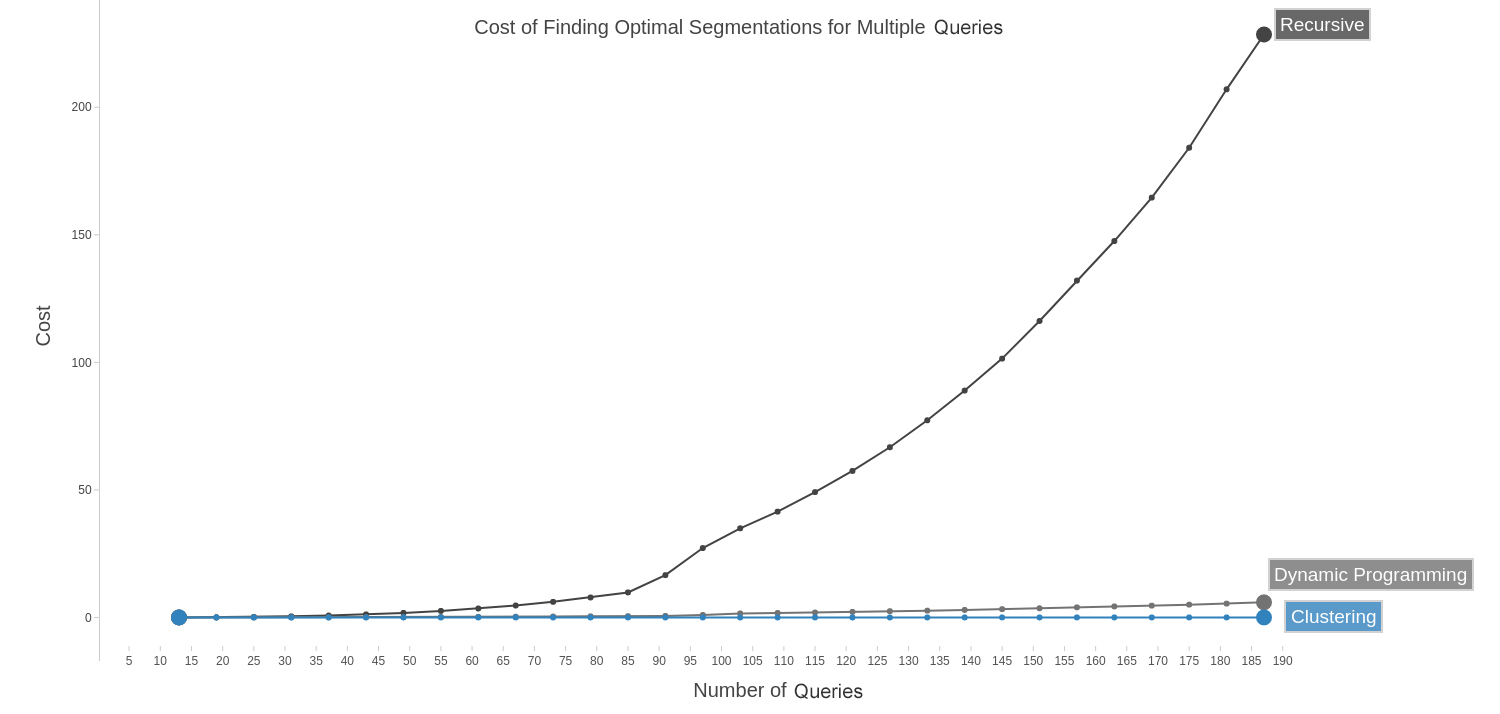
\includegraphics[width=\textwidth]{figs/multi_query.jpg}
				\caption{Optimization time with respect to the number of queries}
				\label{fig:variable_queries}
			\end{figure} 


			\begin {center}
			\begin{table}
				\centering
				\caption{Optimization time with respect to the number of queries}
				\label {table:variable_queries}
				\begin{tabular}{p{2cm}p{3cm}p{3cm}p{3cm}}
					\hline
					Queries & Recursive      & Dynamic  & Clustering \\ \hline
					13 & 0.05   & 0.01  & 0.02  \\  
					43 & 1.23   & 0.13  & 0.03  \\
					73 & 6.15   & 0.39  & 0.03  \\
					103 & 34.98 & 1.60  & 0.03  \\
					133 & 77.31 & 0.69  & 0.04 \\
					163 & 147.57 & 4.35  & 0.04  \\
					187 & 228.52 & 5.96  & 0.04  \\\hline
				\end{tabular}
			\end{table}
			\end{center}

			Figure \ref{fig:variable_queries_2} and Table \ref{table:variable_queries_2} shows that similar to the previous experiment, recursive algorithm has proven to be expensive in computing the optimal timestamps for the snapshots. To see the difference between the dynamic programming and the clustering method, we compared the performance of both in Figure \ref{fig:variable_queries_2} and Table \ref{table:variable_queries_2}. 

			\begin{figure}
				\centering
				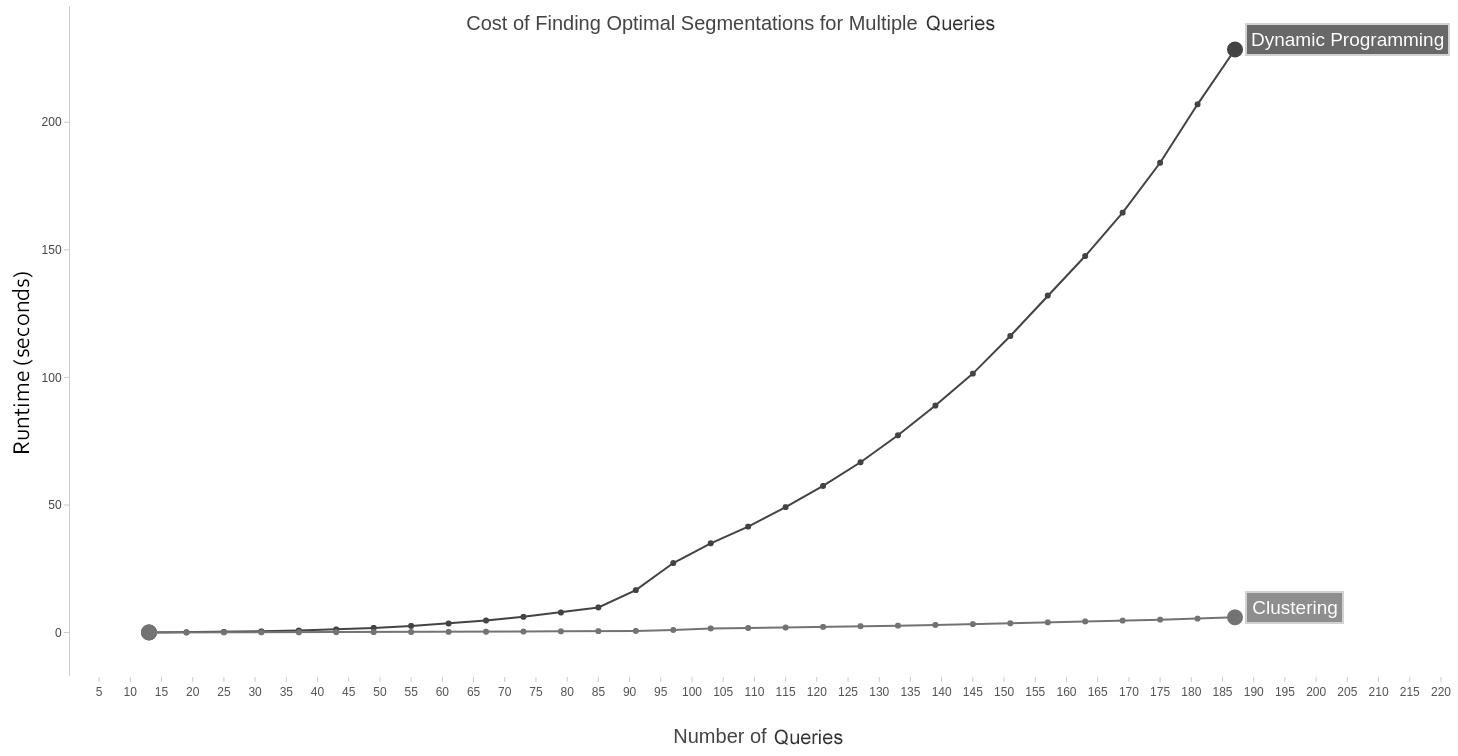
\includegraphics[width=\textwidth]{figs/multi_query_2.jpg}
				\caption{Optimization time with respect to the number of queries}
				\label{fig:variable_queries_2}
			\end{figure} 


			\begin {center}
			\begin{table}
				\centering
				\caption{Optimization time with respect to the number of queries}
				\label {table:variable_queries_2}
				\begin{tabular}{p{2cm}p{3cm}p{3cm}p{3cm}}
					\hline
					Queries  & Dynamic  & Clustering \\ \hline
					13 & 0.01  & 0.02  \\  
					43 & 0.13  & 0.03  \\
					73 & 0.39  & 0.03  \\
					103 & 1.60  & 0.03  \\
					133 & 0.69  & 0.04 \\
					163 & 4.35  & 0.04  \\
					187 & 5.96  & 0.04  \\\hline
				\end{tabular}
			\end{table}
			\end{center}

			The results obtained from these set of experiments show that, for the dynamic programming to find the most optimal timestamps to place snapshots, it takes 21.09 seconds to find 40 number of optimal segmentations from 140 queries. This amount of runtime could be sufficient for the systems in which the {\it{exact optimal}} solution is needed or the computational time is not that important. However, in larger systems with thousands of queries and the need for hundreds of snapshots, the computational time is a very important factor. Mobile systems are also another example in which the runtime matters the most. This motivated us to look into the heuristic method with more favorable runtime.

			\subsection{Evaluating the heuristic method} \label{sec:evaluating_heuristic}
			In the previous section we showed that the heuristic method (K-Means clustering method in this case) is computationally more favorable than the recursive algorithm and dynamic programming method. However unlike recursive algorithm and dynamic programming which compute the exact optimal timestamps for the snapshots, the heuristic method approximates the optimal timestamps. Because of this, in the heuristic method, finding the most optimal timestamps for the snapshots is not guaranteed. Therefore a comparison was needed to evaluate if the heuristic method could be chosen over the other two method.

			We previousely showed that as the number of snapshots grow, the overall cost of answering to the queries drops. In this experiment, we compared the outcome of the dynamic programming and K-Means clustering method in varying number of snapshots to see how increasing the number of snapshots affect the overall cost of query answering in both methods. As it could be seen in Figure \ref{fig:dynamic_vs_heuristic} and Table \ref{table:dynamic_vs_heuristic}, the outcome of dynamic programming and heuristic method is slightly different but the all in all the result of the heuristic method is satisfactory.

			\begin{figure}
				\centering
				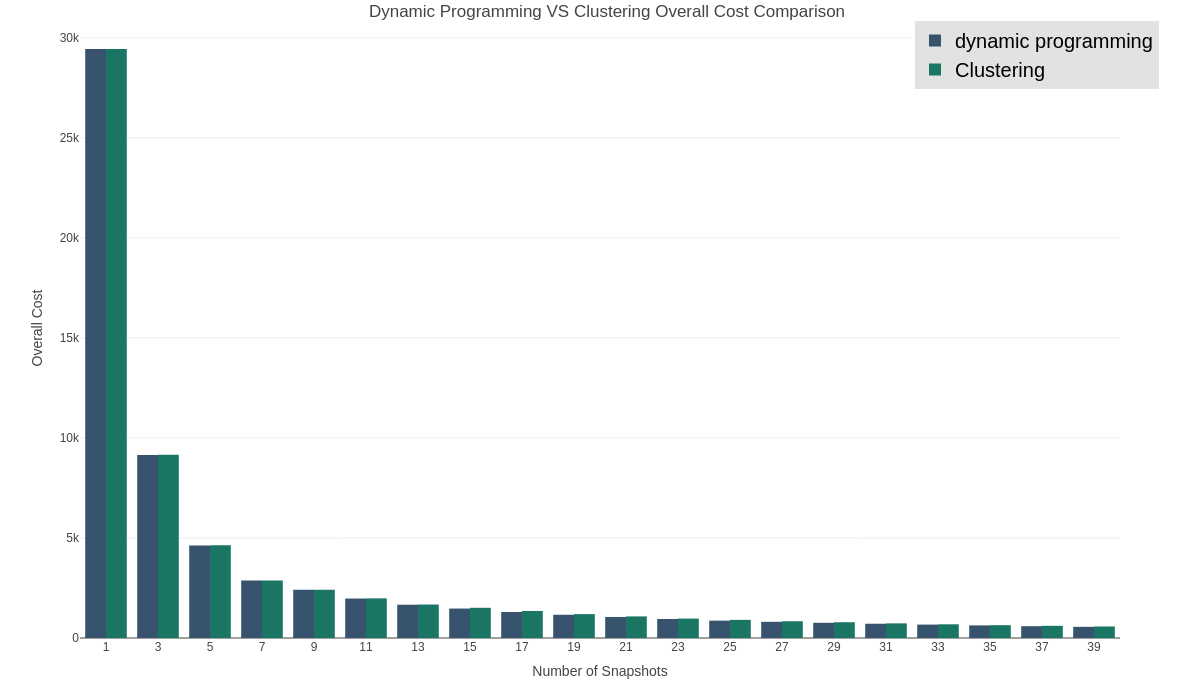
\includegraphics[width=\textwidth]{figs/dynamic_vs_clustering.jpg}
				\caption{Comparing the outcome of dynamic programming with the heuristic method}
				\label{fig:dynamic_vs_heuristic}
			\end{figure} 

			\begin {center}
			\begin{table}
				\centering
				\caption{Comparing the outcome of dynamic programming with the heuristic method}
				\label {table:dynamic_vs_heuristic}
				\begin{tabular}{p{2cm}p{3cm}p{3cm}p{3cm}}
					\hline
					Snapshots & Dynamic  & Clustering \\ \hline
					1 & 29439.26  & 29439.26  \\  
					3 & 9141.55  & 9159.13  \\
					5 & 4626.77  & 4630.08  \\
					7 & 2867.74  & 2867.74  \\
					9 & 2410.46  & 2412.62 \\
					11 & 1972.14  & 1980.95  \\
					13 & 1664.14  & 1673.32  \\
					15 & 1471.58  & 1509.57  \\
					17 & 1300.32  & 1351.44  \\
					19 & 1162.25  & 1194.61  \\
					21 & 1051.97  & 1079.71  \\
					23 & 951.06  & 970.72  \\
					25 & 867.35  & 907.30  \\
					27 & 810.01  & 836.97  \\
					29 & 759.69  & 787.86  \\
					31 & 713.04  & 731.61  \\
					33 & 670.39  & 684.13  \\
					35 & 629.69  & 640.58  \\
					37 & 591.08  & 608.96  \\
					39 & 557.81  & 575.97  \\\hline
				\end{tabular}
			\end{table}
			\end{center}

			The results of K-Means clustering method shown in Figure \ref{fig:dynamic_vs_heuristic} and Table \ref{table:dynamic_vs_heuristic} obtained by performing 300 number of iterations to find the appropriate centroids and clusters from the queries. Although 300 iterations improves the precision of the outcome but we were interested to see if we can lower the number of iterations for the sake of saving more time but still get satisfactory results. Therefore we lowered the number of iterations to 30 and compared the runtime with 300 iterations. Figure \ref{fig:clustering_comparison_multiQuery} shows the runtime comparison of K-Means clustering method with 300 iterations and 30 iterations for fixed number of queries but variable number of snapshots and Figure \ref{fig:clustering_comparison_multiSnap} shows the same comparison for fixed number of snapshots but varying number of queries.

			\begin{figure}
				\centering
				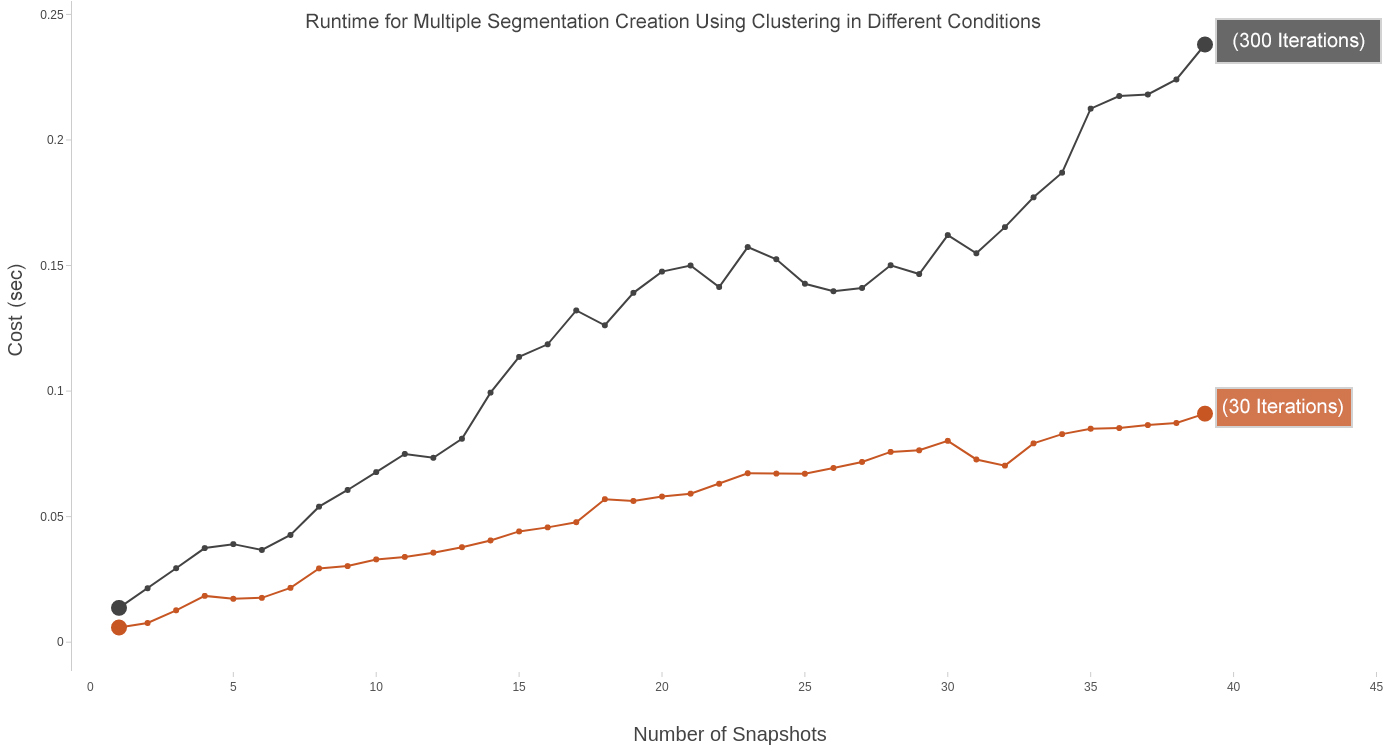
\includegraphics[width=\textwidth]{figs/multiSnap_clustering.jpg}
				\caption{Comparing the runtime of K-Means clustering method with 30 and 300 iterations for variable number of snapshots}
				\label{fig:clustering_comparison_multiSnap}
			\end{figure} 

			\begin{figure}
				\centering
				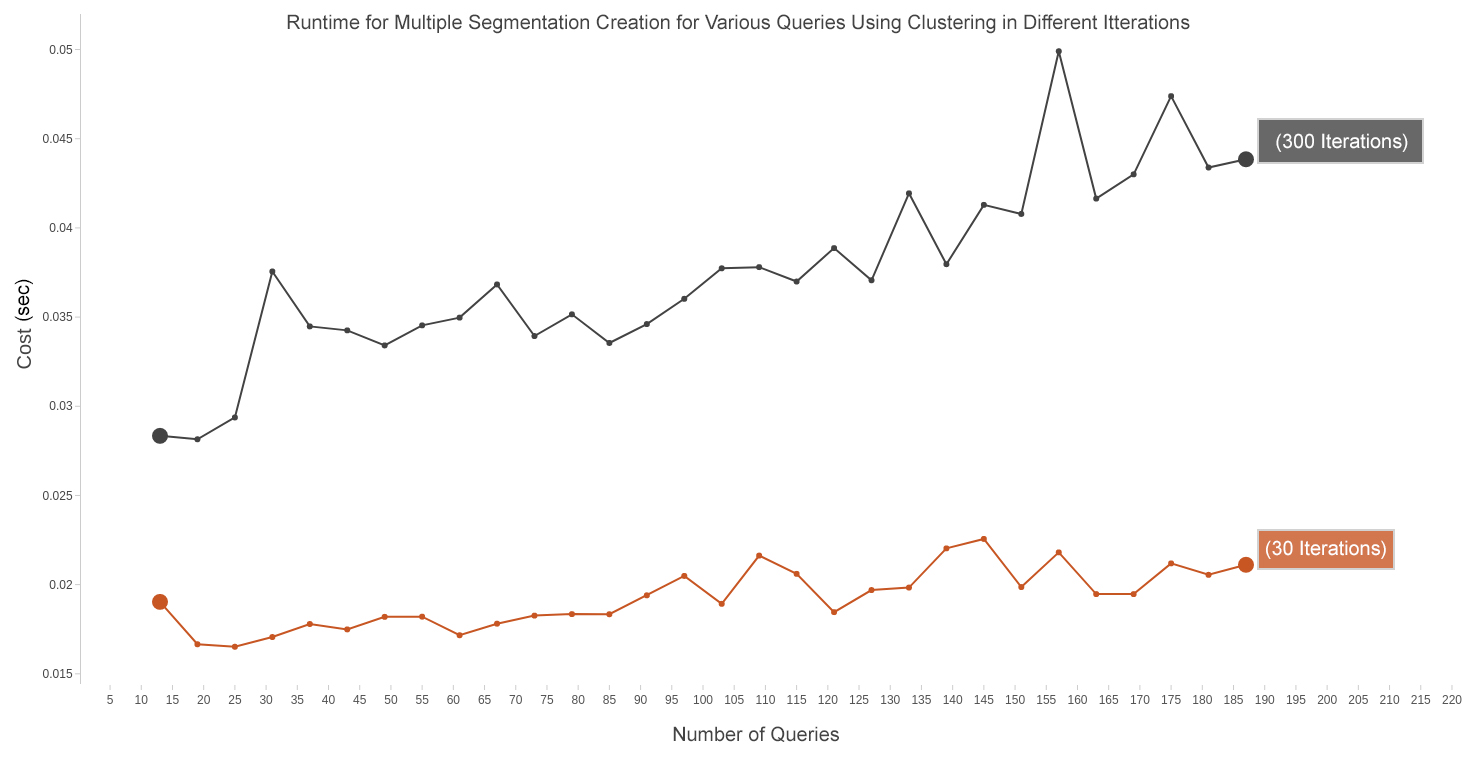
\includegraphics[width=\textwidth]{figs/multiQuery_clustering.jpg}
				\caption{Comparing the runtime of K-Means clustering method with 30 and 300 iterations for variable number of queries}
				\label{fig:clustering_comparison_multiQuery}
			\end{figure} 

			We further lowered the number of iterations to 5 and compared the overal cost of query answering in variable number of snapshots. As seen in Figure \ref{fig:compare_clusterings_iterations} and Table \ref{table:compare_clustring_iterations}, the cost of query answering is more expensive when 5 iterations were used in K-Means clustering however this difference is not significant as the number of snapshots grow.

			\begin{figure}
				\centering
				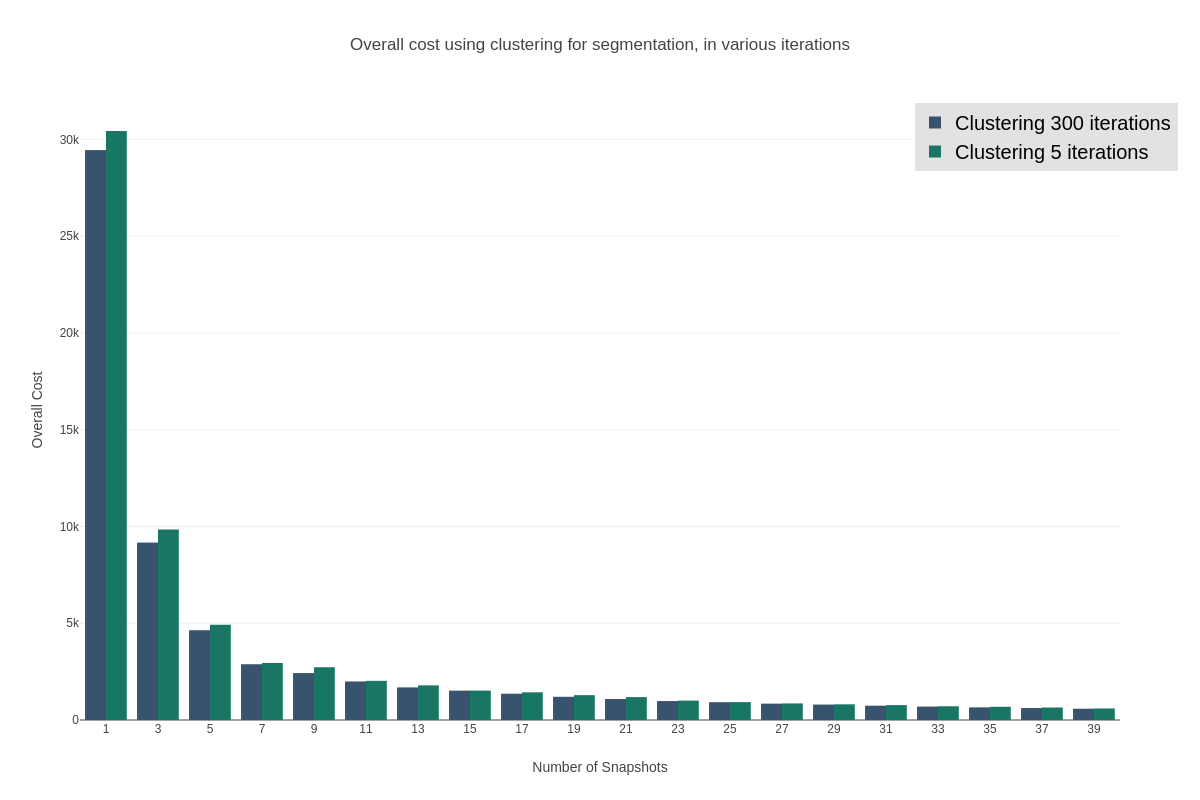
\includegraphics[width=\textwidth]{figs/compare_clustering_iterations.png}
				\caption{Comparing the overal cost of query answering in variable number of snapshots using K-Means clustering method with 30 and 300 iterations to find optimal timestamps for snapshots}
				\label{fig:compare_clusterings_iterations}
			\end{figure} 

			\begin {center}
			\begin{table}
				\centering
				\caption{Comparing the overal cost of query answering in variable number of snapshots using K-Means clustering method with 30 and 300 iterations to find optimal timestamps for snapshots}
				\label {table:compare_clustring_iterations}
				\begin{tabular}{p{2cm}p{3cm}p{3cm}p{3cm}}
					\hline
					Snapshots  & 300 iterations  & 5 iterations \\ \hline
					1 & 29439.26 & 30439.26 \\  
					3 & 9159.13  & 9841.13\\
					5 & 4630.08  & 4921.08\\
					7 & 2867.74  & 2945.76\\
					9 & 2412.62  & 2732.38\\
					11 & 1980.95  & 2023.24\\
					13 & 1673.32  & 1789.50\\
					15 & 1509.57  & 1521.68\\
					17 & 1351.44  & 1430.66\\
					19 & 1194.61  & 1284.61\\
					21 & 1079.71  & 1182.71\\
					23 & 970.72  & 1002.57\\
					25 & 907.30  & 923.30\\
					27 & 836.97  & 856.83\\
					29 & 787.86  & 811.08\\
					31 & 731.61  & 769.83\\
					33 & 684.13  & 710.49\\
					35 & 640.58  & 683.60\\
					37 & 608.96  & 645.74\\
					39 & 575.97  & 595.89\\\hline
				\end{tabular}
			\end{table}
			\end{center}

		\section{Discussion}
			In this chapter the effectiveness of the proposed solutions to both lower the cost of queries on the temporal tables and add transaction transparency to the stored records in a database were put into experiment. We argued that the system could be developed by various tools but in order to generalize the application of our proposed methods for similar systems, we chose the most favorable programming languages and tools by developers.

			The effectiveness of the snapshot materialization was the first set of experiments which was carried out. The experiments proved our claim that for a single snapshot placement for materialization, the median of the perviousely performed queries is the most optimal timestamp. The experiments also showed that for calculating the multiple optimal segmentation of queries on the timeline, the heuristic method beats the recursive and dynamic programming method in terms of computational time complexity. Our experiments showed that although the optimal solution is not guaranteed in the heuristic method, but the results obtained by using this method are satisfactory. For the sake of reducing the computational time even more, we lowered the iteration of the heuristic method and the results obtained were still satisfactory.

			Briefly speaking, the advantages and disadvantages of utilizing recursive algorithm, dynamic programming and heuristic method could be shown in Table \ref{table:segmentation_comparison}. 
			\begin{center}
				\begin{table}
					\centering
					\small
					\caption{Snapshot $s_2$ at $t = 2018-03-15$}
					\label{table:segmentation_comparison}
					\begin{tabular}{p{4cm}p{4cm}p{4cm}}
						\hline
						method & Pros  & Cons  \\ \hline
						Recursive algorithm & Exact optimal solution & computationally expensive for large number of queries and segmentations   \\ \hline
						Dynamic programming & Exact optimal solution & computationally expensive for large number of queries and segmentations\\ 
						  & Computationally cheaper than dynamic programming &    \\ \hline
						K-Means clustering & Fast in computation & optimal solution not guaranteed \\ \hline
					\end{tabular}
				\end{table}
			\end{center}
			
\chapter{Conclusion}

	\section{Summary}
		In this work, implementation of a Blockchain based tool was proposed which works on top of the Relational Database Management System (RDBMS) and ensures the trustworthiness of the records that are stored in the relational database tables. This system follows a mechanism to store the historical records of the transactions on the relational tables in the temporal databases which can be used as a source of data provenance for the database system. To implement the system, two major problems was identified: 
		\begin{itemize}
			\item Lower the cost of queries performed on the temporal database.
			\item Add data transparency to the stored reocords in the temporal table.
		\end{itemize}

		The problem of linear time and storage to perform queries on the temporal databases shown both theoretically and experimentally. In the presence of multiple and concurrent queries on the temporal table, performing such queries are inefficient and infeasable. To solve this problem, the materialization of multiple precomputed snapshots proposed. The proposed method advices that keeping the timestamp of previous queries which was performed on the temporal table
		gives insight into the pattern of queries on the table and identifies hotspots that subsequent queries have high chance of falling into. Optimal segmentation of the performed queries, clusters the hotspots and specify a precomputed snapshot for each cluster to materialize. It is expected that this method result in lowering the overall cost of query answering on the temporal database.

		For the placement of a single snapshot for materialization, both mathematical and experimental approach showed that the most optimal timestamps is the median of previousely performed queries. This notion could be extended for placing multiple precomputed snapshots for materialization, in the sense that when optimal multiple segmentations of the queries were computed, the optimal place in each segmentation for placing the snapshot is the median of queries in that segment.

		Finding the optimal multiple segmentations of the previousely performed queries was performed using three different aproaches: recursive algorithm, dynamic programming and heuristic method. The experiments showed that although the heuristic method does not guarantee the most optimal solution, but because of less computational time in comparison with other two methods and returning satisfactory results, it is more favorable to be utilized in this project.

		Using Blockchain to add record transparency of temporal tables, require these tables to have a few mandatory attributes: the transaction submitters information, the digital signature of the record signed by transaction submitter's cryptoraphic keys and the previous record's digital signature. Having the digital signature of the previous record chains the submitted records together and makes any malicious or accidental record modification evident.

		The validation of the chain of records is done by
		\begin{itemize}
			\item making sure that the current record's \it{'previous signature'} matches the previous record's \it{'current signature'} attribute for all the records in the table.
			\item validate the signature of every single record by using the transaction submitters cryptographic keys.
		\end{itemize}
		
		This procedures are expensive and contradicts the idea of snapshot materialization that we discussed earlier. To solve the problem, it is recommended to create a digital signature of the precomputed snapshots, then the validation of the chain of records is done by:
		\begin{itemize}
			\item check the digital signature of the snapshot that the query is materializing.
			\item for the records that fall in between the query timestamp and snapshot timestamp, use the manual chain validation technique
		\end{itemize}

		Digitally signing the snapshots require the system to check the authenticity of the records that are stored in it beforehand. This procedure requires the system to manually check the validation of the chain of records. This is an expensive procedure, specially for the snapshots that are placed at the end of the timeline. To reduce the cost, it was proposed that the manual chain validation to be performed for the first snapshot and the subsequent snapshots materialize their previous snapshot for chain validation.

	\section{Conclusion}
	In this thesis, in order to establish a trusted temporal relational database, the use of historical data as a source of data provenance is suggested. Data provenance sources can hold useful evidences about the legitimacy of a record throughout its lifecycle in a database system. Temporal databases are a good candidate to store the historical data on becuase it gives us a systematic way to work with the historical data. Since the temporal databases are not immune from malicious attacks, it is required that the data stored in them to be immutible, and any attempts for a forgery on their records to be computationally expensive and evident. Digital signature not only guarantees the immutability of the records in a database, but also is a verifiable evidence to show that the transaction has been authenticated. This makes digital signatures as a perfect tool to guarantee the immutability of the records in the source of data provenance. To reduce the risk of adverserial attacks, the records that are digitally signed could be chained together by a record holding its previous record's digital signature. This makes any malicious or accidental modification of the records evident.
	Append-only temporal databases can become massive as they store all the updates on the relations of a database. This makes querying on the temporal database expensive as there is a need to compute a large workload for each query. Snapshot materialization is a suitable way to reduce the cost of query answering on the temporal databases. If the right number of snapshots chosen, and they placed in optimal timestamps for materialization, not only the cost of answering to the queries can be reduced, but also the verification of the authenticity of chains of records can be done in a much faster way.
	\section{Future work and other remarks}
		Possible extensions that could be added are: adding the revision functionality in which the maliciousely altered records are revised to their previous form. The application of the work is endless and it ranges from ordinary relational database of an enterprise, to the databases of the social media and it could be used to find th origin of a submitted post in these mediums.

%----------------------------------------------------------------------------------------
%	THESIS CONTENT - APPENDICES
%----------------------------------------------------------------------------------------

%\appendix % Cue to tell LaTeX that the following "chapters" are Appendices

% Include the appendices of the thesis as separate files from the Appendices folder
% Uncomment the lines as you write the Appendices

%\include{Appendices/AppendixA}
%\include{Appendices/AppendixB}
%\include{Appendices/AppendixC}

%----------------------------------------------------------------------------------------
%	BIBLIOGRAPHY
%----------------------------------------------------------------------------------------

\printbibliography[heading=bibintoc]

%----------------------------------------------------------------------------------------

\end{document}  
